\chapter{Cosmology}

\section{Homogeneous and Isotropic Cosmology - GR perspective}
\subsection{Spherically-symmetric space-times}
Physical cosmology aims at studying the structure and evolution of the
universe as a whole. Of the four fundamental interactions of physics,
only gravity is relevant on the largest scales because the strong and
the weak interactions are confined to sub-atomic length scales, and the
electromagnetic force is shielded on large scales by opposite charges.
We thus expect that the space-time of the Universe can be idealised as
a solution of Einstein’s field equations, satisfying certain simplicity requirements expressed by symmetries imposed on the form of the solution.
In this chapter, we shall therefore first discuss spherically-symmetric
space-times in general and then specialise them to cosmological solutions
in particular.

\subsubsection{Form of the metric}
Generally, a space-time (M, g) is called \emph{spherically symmetric} if it admits
the group $SO(3)$ as an isometry such that the group’s orbits are two-
dimensional, space-like surfaces. Space-like hypersurface means that all normal vectors of these hypersurfaces are time-like, or that the corresponding tangent vectors are space-like.
For any point $p \in M$, we can then select the orbit $Ω(p)$ of $SO(3)$ through
$p$. In other words, we construct the spatial two-sphere containing $p$
which is compatible with the spherical symmetry. I.e. take $p\in M$, construct orbit around $p\Rightarrow$ get a sphere. This is the group orbit of $\Omega(p)$. On this sphere use coordinates $(\vartheta, \varphi)$.

\begin{figure}[h!]
	\centering
	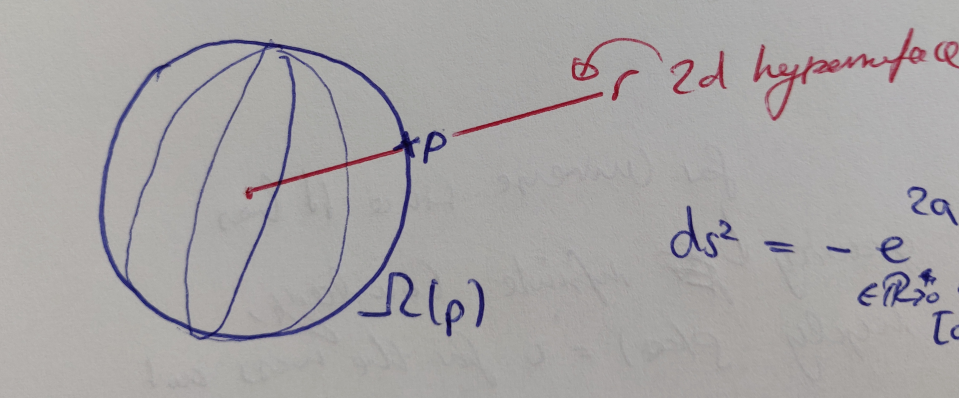
\includegraphics[width=0.7\linewidth]{gfx/SphericallySymmetricSpacetime}
	\caption{\itshape Group orbits around point make up $S^2$, the orthogonal space is $N(p)$.}
	\label{fig:sphericallysymmetricspacetime}
\end{figure}

Next, we construct the set of all geodesics $N(p)$ through $p$ which are
orthogonal to $Ω(p)$. Locally, $N(p)$ forms a two-dimensional surface
which we also call $N(p)$. Repeating this construction for all $p \in M$
yields the surfaces $N$.
We can now introduce coordinates $(r, t)$ on $N$ and $(θ, φ)$ on $Ω$, i.e. such
that the group orbits $Ω$ of $SO(3)$ are given by $(r, t) = const.$ and the
surfaces $N$ by $(θ, φ) = const.$ With these adapted coordinates, the metric has the following line element.
\begin{mybox}{Metric of a spherically-symmetric space-time}
	The line element of the metric of a spherically-symmetric space-time
	M can be written in the form
	\begin{equation}
	\md s^2 = \md \tilde{s}^2 + R(t,r) \md \Omega^2
	\end{equation}
	where $\md \tilde{s}^2$ is the line element of a yet unspecified metric $\tilde{g}$ in the
	coordinates $(t, r)$ on the surfaces $N$. This is equivalently derived from the theory of maximally symmetric spaces in \ref{eq:metricsphericallysymmetricspacetime}
	Without loss of generality, we can now choose $t$ and $r$ such that the
	metric $\tilde{g}$ is diagonal, which allows us to write its line element as
	\begin{equation}
	\md \tilde{s}^2 = -e^{2a(t,r)} \md t^2 +e^{2 b(t,r)} \md r^2
	\end{equation}
	with functions $a(t, r)$ and $b(t, r)$ to be determined, now time-dependent !
\end{mybox}
The chosen dual basis then is
\begin{equation}
\theta^0 = e^a \md t, \, \theta^1 =e^b \md r, \; \theta^2 = R \md \vartheta, \; \theta^3 = R \sin \vartheta \md \varphi.
\end{equation}


\subsubsection{Generalised Birkhoff's theorem}
\begin{mybox}{Birkhoff's generalized theorem}
	Every $C^2$ solution of Einstein’s vacuum equations which is spherically
	symmetric in an open subset $U \subset M$ is locally isometric to a domain
	of the Schwarzschild-Kruskal solution.
\end{mybox}
Now we don't want a static or stationary solution, we don't have a preffered time direction. 
\begin{mybox}{Cavity in spherically-symmetric space-time}
	It is a corollary to Birkhoff’s theorem that a spherical cavity in a
	spherically-symmetric spacetime has the Minkowski metric. Indeed,
	Birkhoff’s theorem says that the cavity must have a Schwarzschild
	metric with mass zero, which is the Minkowski metric.
\end{mybox}


\subsection{Homogeneous and Isotropic Space-times}
There are good reasons to believe that the Universe at large is \emph{isotropic}
around our position. The most convincing observational data are provided by the cosmic microwave background, which is a sea of black body
radiation at a temperature of $(2.725 ± 0.001) K$ whose intensity is almost
exactly independent of the direction into which it is observed.\\
\\
There is furthermore no good reason to believe that our position in the
Universe is in any sense preferred compared to others.  This is known as the \emph{Cosmological Principle}: all positions in the universe are essentially equivalent. The Cosmological Principle can be formulated as a statement about the existence of equivalent coordinate systems. A different set of space-time coordinates $x^{\prime \mu}$ must be \emph{equivalent} to some fiducial cosmic standard coordinates $x^\mu$ (the fiducial coordinate frame of the CMB), if the whole history oft he universe appears the same in the $x^{\prime \mu}$ as in the fiducial coordinate system $x^\mu$ This simply says that the coordinate transformation $x^\mu\rightarrow x^{\prime\mu}$ must be an \emph{isometry} and than the tensors $g\munu, T\munu$ must be \emph{form-invariant} under this transformation. We must therefore
conclude that any observer sees the cosmic microwave background as an isotropic source such as we do. Then, the Universe must also be
\emph{homogeneous}.\\
\\
We are thus led to the expectation that our Universe at large may be
described by a homogeneous and isotropic space-time. Let us now give
these terms a precise mathematical meaning.
\begin{mybox}{Spatially homogeneous space-time}
	A space-time $(M, g)$ is called \emph{spatially homogeneous} if there exists a
	one-parameter family of space-like hypersurfaces $\Sigma_t$ that foliate the
	space-time such that for each $t$ and any two points $p, q ∈ \Sigma_t$ , there exists
	an isometry $φ$ of $g$ which takes $p$ into $q$.\\
	$"g(q) = g(q+p)"$.
\end{mybox}
\begin{figure}[h!]
	\centering
	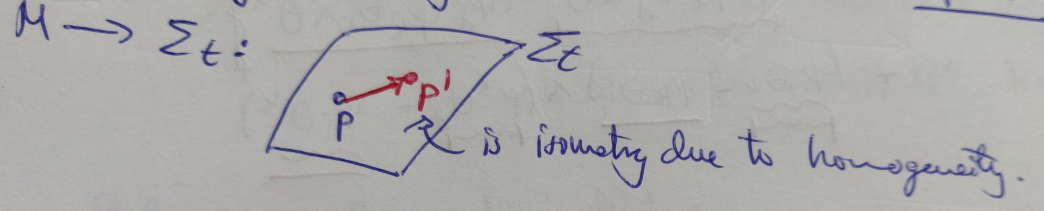
\includegraphics[width=0.7\linewidth]{gfx/HomogeneousSpacetime}
	\caption{\itshape The isometry is a translation relating points on the space-like hypersurface.}
	\label{fig:homogeneousspacetime}
\end{figure}




Before we can define isotropy, we have to note that isotropy requires that
the state of motion of the observer needs to be specified first because two
observers moving with different velocities through a given point in space-
time will generally observe different redshifts in different directions. Spatial isotropy is thus observer dependent.
\begin{mybox}{Spatially isotropic space-time}
	Therefore, we define a space-time $(M, g)$ as spatially isotropic about a
	point $p$ if there exists a congruence of time-like geodesics through $p$
	with tangents $u$ such that for any two vectors $v_1 , v_2 \in T_p M$ orthogonal
	to $u$, there exists an isometry of $g$ taking $v_1$ into $v_2$ but leaving $u$ and
	$p$ invariant. In other words, if the space-time is spatially isotropic, no
	preferred spatial direction orthogonal to $u$ can be identified.\\
	\\Caroll:More formally, a manifold $M$ is isotropic around a point $p$ if, for any two vectors $V$ and $W$
	in $T_p M$, there is an isometry of $M$ such that the pushforward of $W$ under the isometry is
	parallel with $V$ (not pushed forward).
\end{mybox}
\begin{figure}
	\centering
	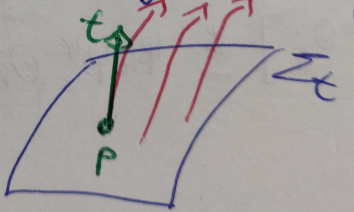
\includegraphics[width=0.7\linewidth]{gfx/IsotropicSpacetime}
	\caption{\itshape The space-time is isotropic w.r.t. the preferred flow defining a bundle of time-like geodesics which are related by isometries.}
	\label{fig:isotropicspacetime}
\end{figure}


Isotropy thus identifies a special class of observers, with four-velocities
$u$, who cannot identify a preferred spatial direction. The spatial hypersurfaces $\Sigma_t$ must then be orthogonal to $u$ because otherwise a preferred
direction could be identified through the misalignment of the normal
direction to $\Sigma_t$ and $u$, breaking isotropy.\\
All coordinates systems that are equivalent to the fiducial cosmic standard system necessarily use cosmic standard time. The assumption of spatial isotropy can therefore equivalently following Weinberg be formulated as the requirement that there exists a family of coordinate systems $x^{\prime \mu}(x;\theta)$, depending on the three independent parameters $\theta^1,\theta^2,\theta^3$, which are equivalent to the cosmic standard coordinates, and which have the same origin, that is,
\begin{equation}
x^{\prime i}(0,t;\theta)=0
\end{equation}
We can intuitively think of the three parameters $\theta^n$ as Euler angles that specify the orientation of the $x^{\prime i}$ coordinate axes relative to the $x^i$ coordinate axes of the fiducial system; the important thing is that there be \emph{three} independent parameters. (In formulating this assumption, we have \textbf{tacitly assumed that the privileged Lorentz frame in which the universe appears isotropic happens to coincide more or less with the origin of the fiducial coordinate system, which is the CMB}.)
\\
Formulating the assumption of homogeneity: Clearly, homogeneity does not mean that any object can be chosen as the origin of a coordinate system equivalent to our cosmic standard coordinates -  after all, the universe looks different to an observer moving away from the Liky Way at half the speed of light than it does to us. The most we can expect is that every point $x^\mu$ in space-time is on some "fundamental  trajectory" $x^i=X^i(t)$ (Hubble flow), which can serve as the origin of a coordinate system $x^{\prime \mu}$ equivalent to the cosmic standard system. The important point is that, since the $\vec{X}(t)$ at any time $t$ fill up all space, they are determined by \emph{three} independent parameters $a^i$. Thus homogeneity means that there is a three-parameter set of cordinates $\bar{x}^{\prime \mu}(x;a)$, which are equivalent to the cosmic standard coordinates $x^\mu$, and which have origin on the trajectory $x^i=X^i(t;a)$, that is,
\begin{equation}
\bar{x}^{\prime i}(\vec{X}(t;a),t;a) =0.
\end{equation}
To be more precise, the $\vec{X}(t;a)$ are \emph{the trajectories of the privileged observers to whom the universe appears isotropic}, i.e. \emph{observers comoving with the Hubble flow.}
\\
We thus arrive at the following conclusions: a homogeneous and isotropic
space-time $(M, g)$ is foliated into space-like hypersurfaces $\Sigma_t$ on which $g$
induces a metric $h$. There must be isometries of $h$ carrying any point $p \in \Sigma_t$ into any other point $q \in \sigma_t$ . Because of isotropy, it must furthermore	be impossible to identify preferred spatial directions on $\Sigma_t$ . These are
very restrictive requirements which we shall now exploit.
\subsubsection{Assumptions imply Killing vectors}
Putting the above together, we see that the Cosmological Principle entails the existence of two independent three-parameter families of coordinate transformation $x\rightarrow x^\prime$, $x\rightarrow\bar{x}^\prime$, which are isometries and which leave the time coordinate invariant. Descend to the case of infinitesimal transformations, letting $a^i, \theta^i$ approach zero, lets us find six "Killing vectors" $\xi^\mu_j(x)$ and $\bar{\xi}^\mu_j(x)$, defined by
\begin{align}
	\label{eq:cosmologicalKillingVectors}
	\xi^i_j(x) & \equiv \frac{\partial x^{\prime i}(x;\theta)}{\partial \theta^j} |_{\vec{\theta}=0} \qquad  \xi^t_j(x)\equiv=0\\
	\bar{\xi}^i_j(x) &\equiv \frac{\partial \bar{x}^{\prime i} (x;a)}{\partial a^j} |_{\vec{a}=0} \qquad \bar{\xi}^i_j(x)\equiv 0.
\end{align}
Thus we have six independent Killing vectors with $\xi^t=0$, the maximum number possible in three dimensions. The universe therefore satisfies the requirements for a four-dimensional space with three-dimensional maximally symmetric subspaces $\Sigma_t$ with $t=$constant.\\
The cosmological Principle can therefore be formulated in the language of Maximally symmetric spaces as follows:
\begin{enumerate}
	\item The hypersurfaces with constant cosmic standard time are maximally symmetric subspaces of the whole space-time.
	\item Not only the metric $g\munu$, but all cosmic tensors such as $T\munu$ are form-invariant w.r.t. the isometries of these subspaces.
\end{enumerate}





\subsubsection{Line of Reasoning - Weinberg}
The Cosmological Principle allows the specification of the cosmic metric entirely in terms of a "radius" $R(t)$ and a trichotomic constant $k$, as in \ref{eq:metricRobertsonWalkerViaMaximalSymmetry}, and we shall then see how astronomical observations can be interpreted as measurement of $R(t)$ and $k$.\\
This inherently kinematic approach, pioneered in the 1930's by Robertson and Walker, is incomplete in that it does not provide and \emph{a priori} prediction of the function $R(t)$. To calculate $R(t)$ we need to make some assumption about the material content of the universe, and then derive the Robertson-Walker metric as a solution of the Einstein field equations \ref{eq:metricRobertsonWalkerViaField}, as first done by Friedmann in 1922.\\
\\
Weinberg makes the distinction to call this section cosmography and later discussion on the contents of the universe cosmology, why this distinction between cosmography and cosmology ? The reason is simply that we do not know the equation of state of the matter and radiation of the universe throughout its history, and even if we did, we could not be sure that the Einstein equations really hold over cosmic times and distances. A modification of the field equations or the equations of state, such as the introduction of a cosmological constant, or a large population of gravitons, \emph{would affect $R(t)$ and invalidate the simplest Friedmann solution, but it wuld not require us to make any change in the descriptive framework assembled in this chapter}.\\
\emph{If the data of observations will not fit into this framework, we shall be able to conclude that either the Cosmological Principle or the Principle of Equivalence is wrong. Nothing could be more interesting.}








\subsubsection{Spaces of constant curvature}
Consider now the curvature tensor $^{(3)}\bar{R}$ induced on $\Sigma_t$  (i.e. the curvature
tensor belonging to the metric $h$ induced on $\Sigma_t$ ):
\begin{equation}
^{(3)} \bar{R} = ^{(3)}\bar{R}^{\;\, kl}_{ij}.
\end{equation}
In this way, $^{(3)} \bar{R}$ represents a linear map from the vector space of 2-forms $\bigwedge^2$into $\bigwedge^2$ , because of the antisymmetry of $^{(3)}\bar{R}$ with respect to
permutations of the first and the second pairs of indices. Thus, it defines
an endomorphism:
\begin{equation}
L:\bigwedge^{\,2} \rightarrow \bigwedge^{\,2}, \quad ^{(3)} \bar{R}^{\,\,kl}_{ij} \omega_{kl} = (L\omega)_{ij} \, \in \bigwedge^2.
\end{equation}
Due to the symmetry of $^{(3)}\bar{R}$ upon swapping the first with the
second pair of indices, the endomorphism $L$ is self-adjoint. In fact, for any pair of 2-forms $α, β \in \bigwedge^2: \langle \alpha, L \beta \rangle = \langle \beta, L \alpha>$. Every self-adjoint endomorphism defines an orthonormal set of eigenvectors (3 of them), which have all the same eigenvalue by isotropy assumption:
\begin{equation}
L = id \cdot 2 k
\end{equation}
where $k$ is the \emph{spatial curvature parameter}.
Then, by this endomorphism the induced spatial curvature still has to be antisymmetric in both index pairs:
\begin{equation}
^{(3)}\bar{R}_{ij}^{kl} = k \left[\delta^k_i \delta^l_j - \delta^k_j \delta^l_i \right]\, \Rightarrow \, ^{(3)}\bar{R}_{ijkl} = k \left[h_{ik} h_{jl} - h_{jk} h_{il}\right],
\end{equation}
where the indices where lowered by means of the induced metric $h$. Then
\begin{equation}
^{(3)}R_{jl} = 2 k h_{jl} \quad \Rightarrow \quad ^{(3)} \mathcal{R}= 6 k.
\end{equation}
The curvature forms are then found to be
\begin{equation}
\Omega^i_j = \frac{1}{2} ^{(3)} \bar{R}^i_{jkl} \theta^k \wedge \theta^l = k \theta^i \wedge \theta_j.
\end{equation}

The curvature parameter k must be (spatially) constant because of homogeneity.
\begin{statements}
	Space-times with constant curvature can be shown to be
	conformally flat.
\end{statements}
This means that coordinates can be introduced in
which the line element $dl^2$ of the metric $h$ reads
\begin{equation}
\md l^2 = \frac{1}{\psi^2} \sum_{i=1}^{3} (\md x^i)^2.
\end{equation}
The modus operandi is now to fix the conformal factor $\psi$ such that $\md l^2$ and $\Omega^i_j$ agree: \\
Start as always by introducing cotetrad to have a Euclidean metric.  The isotropy of our coordinates implies that
\begin{equation}
\psi = \sum_{k=1}^{3} f_k(x^k).
\end{equation}
Catan's structure equations then yield an equation for $\psi$ and $f_k$ such that one finds with $\sum_{i=1}^{3} (x^i)^2=r^2$ and with a specific choice of coordinates
\begin{equation}
\md l^2 = \frac{\sum_i (\md x^i)^2}{\left[1+\frac{k}{4} r^2\right]^2}
\end{equation}
\todo{ Include derivation of curvature forms, how you identify the $k$ and then derive geometric tensors.}
\subsection{Friedmann's equations}
\subsubsection{Connection and curvature forms}
This yields the metric of the four-dimensional space-time. Use the order parameter $t=const.$ of our spatial hypersurfaces $\Sigma_t$ as our time coordinate and choose coordinates such that $g_{00}=1$ and $g_{0i}=0$. Metric doesn't have to look like that, but we choose it such that the former conditions are satisfied.	
\begin{mybox}{Robertson-Walker metric}
	According to the preceding discussion, the homogeneous and isotropic
	spatial hypersurfaces $\Sigma_t$ must have a metric $h$ with a line element of the
	form
	\begin{equation}
	\md l^2 = \frac{\sum_{i=1}^{3}(x^i)^2}{\left(1+\frac{r^2k}{4}\right)^2}, \quad r^2 \equiv \sum_{i=1}^{3} (x^i)^2.
	\end{equation}
	By a suitable choice of the time coordinate $t$, the line element of the
	metric of a spatially homogeneous and isotropic space-time can then
	be written as
	\begin{equation}
	\label{eq:metricRobertsonWalkerViaField}
	\md s^2 = -c^2 \md t^2 + a^2(t) \md l^2
	\end{equation}
	because the scaling function $a(t)$ must not depend on the $x^i$ in order to
	preserve isotropy and homogeneity. This metric  of a spatially
	homogeneous and isotropic space-time is called \emph{Robertson-Walker}
	metric.
\end{mybox}
\begin{mybox}{Alternative forms of the metric}
	We thus find that the homogeneous and isotropic class of cosmological
	models based on Einstein’s field equations are characterised by the line
	element
	\begin{equation}
	\md s^2 = -c^2 \md t^2 + a^2(t) \left[\md \omega^2 + f^2_k(\omega) \left(\md \vartheta^2 + \sin^2 \vartheta \md \varphi^2\right)\right]
	\end{equation}
	with 
	\begin{equation}
	f_k(\omega)=\left\{	\begin{array}{lr}
	{k}^{- \half} \sin(k^{\half} \omega) & \mathrm{if} \, k>0\\
	\omega 												& 			\mathrm{ if} \, k=0 \\
	\abs{k}^{- \half} \sinh( \abs{k}^{ \half} \omega) & \mathrm{if} \, k<0.
	\end{array}			\right\}
	\end{equation}
	which is equivalent to
	\begin{equation}
	\md s^2 = -c^2\md t^2 + a^2(t) \left[ \frac{\md u^2}{1 - k u^2} +u^2\left( \md \vartheta^2 + \sin^2\vartheta \md \varphi^2 \right)\right]
	\end{equation}
	with $u$ related to $\omega$ by $u=f_k(\omega)$, and the scale factor $a(t)$ satisfies the
	Friedmann equations.
\end{mybox}
In a suitable tetrad, we find the geometric tensor quantities by Cartan's structure equations:
\begin{mybox}{Einstein tensor for a spatially homogeneous and isotropic
		space-time}
	The Einstein tensor of a spatially homogeneous and isotropic space-
	time has the components
	\begin{align}
		G_{00}&= 3\frac{k+\dot{a}^2/c^2}{a^2}, \quad G_{11}=G_{22}=G_{33} =-\frac{2 \ddot{a}}{a c^2}- \frac{k+\dot{a}^2/c^2}{a^2} \\
		\mathcal{R} &= 6 \left(\frac{\ddot{a}}{a c^2} + \frac{k+\dot{a}^2/c^2}{a^2}\right)\\
		R_{00}& =- \frac{3 \ddot{a}}{a c^2}, \; R_{11}=R_{22}=R_{33}=\frac{\ddot{a}}{a c^2} + 2\frac{k+\dot{a}^2/c^2}{a^2}.
	\end{align}
\end{mybox}
\subsubsection{On the Robertson-Walker metric - Weinberg}
As for the treatment of maximally symmetric subspaces, we see that the cosmological symmetries allows us to arrive at the Robertson-Walker metric \ref{eq:metricRobertsonWalkerViaMaximalSymmetry}, where the time coordinate appearing $t$ is the standard cosmic time, but could also be a function of it.\\
Note that for $k=-1$ or $k=0$ the space is infinite, while for $k=+1$ it is finite (though unbounded).\\
For $k=+1$ the spatial universe can be regarded as the surface of a sphere of radius $R(t)$ in four-dimensional Euclidean space, and $R(t)$ can justly be called the "radius of the universe". $R(t)$ sets the scale of the geometry of the space, so $R(t)$ will in all cases be called the \emph{cosmic scale factor}, i.e. $R(t)\equiv a(t)$.
\\
\\
Fixing the trajectories of comoving observers by attaching them to the Hubble flow, we can conclude that the spatial coordinates $r,\theta,\phi$ form a \emph{comoving system}, in the sense that \emph{typical galaxies have constant spatial coordinates} $r,\theta,\phi$. One can imagine the comoving coordinate mesh to be like lines painted on the surface of a balloon, on which dots represent typical galaxies. As the balloon is inflated or deflated the dots will move, but the lines will move with them, so each dot will keep the same coordinates.\\
\\
It is important to note that the fundamental (comoving) trajectories $\vec{x}=$constant are geodesics, because \ref{eq:metricRobertsonWalkerViaMaximalSymmetry} gives
\begin{equation}
\Gamma^\mu_{tt} = 0.
\end{equation}
Thus the statement that a galaxy has constant $r,\theta,\phi$ is perfectly consistent with the supposition that galaxies are in free fall. Note also that the time coordinate $t$ in \ref{eq:metricRobertsonWalkerViaMaximalSymmetry} is not only a possible "cosmic standard" time; it is also the proper time told by a clock at rest in any typical freely falling galaxy. The coordinates $x,t$ are thus co-moving in precisely the same sense as the Riemannian normal coordinates.\\
The four-velocity of such a freely-falling or comoving observer is
\begin{equation}
U^t\equiv 1, \qquad U^i \equiv 0.
\end{equation}
This shows that \emph{the contents of the universe are, on the average, at rest in the coordinate system} $r,\theta,\phi$. Furthermore, one can from the comoving observer deduce that \emph{the energy-momentum tensor of the universe necessarily takes the same form as for a perfect fluid.}





\subsubsection{From Einstein to Friedmann}
For Einstein’s field equations to be satisfied, the energy-momentum
tensor must be diagonal, and its components must not depend on the
spatial coordinates in order to preserve isotropy and homogeneity. Spatial isotropy implies a preferred velocity field, together with spatial homogeneity one has one possible choice to built a rank $(0,2)$ tensor we need  by this preferred field: $u^{\flat} \otimes u^{\flat}$, the other symmetric $(0,2)$ tensor is $g$. Every other rank $(0,2)$ would have own set of eigenvectors, thus it would define a preferred direction in conflict with isotropy. We
set $T_{00} = ρc^2$ , which is the total energy density, and $T_{ij} = p δ_{i j}$ , where $p$
is the pressure.
This corresponds to the energy-momentum tensor of an ideal fluid,
\begin{equation}
T = (\rho c^2 + p) u^{\flat} \otimes u^{\flat}\quad + p g.
\end{equation}
In our adapted coordinates, $u^{\flat} = \md t$ and $g$ is Minkowskian. As seen by a fundamental observer (i.e. an observer for whom the spatial
hypersurfaces are isotropic). For such an observer, $u = \partial_t$ , and since the
metric is Minkowskian in the suitable tetrad we find
\begin{equation}
T = (\rho c^2+p) \md t\otimes \md t+ pg, \quad \left\{	\begin{array}{lr}
T_{00} = T(\partial_t,\partial_t) = \rho c^2 \\
T_{11} = p = T_{22} = T_{33},
\end{array}		\right\}
\end{equation}
where $\rho,p = \rho(t), p(t)$ only by isotropy. Equivalently, 
\begin{equation}
u^\mu= \partial_t=(1,0,0,0) \; \Rightarrow \quad T\munu=\begin{pmatrix}
\rho c^2 &0&0&\\
&&&&\\
&&g_{ij} p&&\\
&&&&
\end{pmatrix}.
\end{equation}
Which has the forms
\begin{equation}
T^\mu_\nu = \mathrm{diag}\left(-\rho c^2,p,p,p\right),\quad T= \tr T = -\rho c^2+ 3p.
\end{equation}
Does it follow from here that for $\tr T=0=-\rho c^2+3p$ $\Leftrightarrow p=\frac{\rho c^2}{3}$ for ultra-relativistic matter ? Answer: Radiation and ultra-relativistic matter both are called radiation and they both describe a perfect fluid. hence the adhere to this energy-momentum tensor. At the same time, radiation adheres to the energy-momentum tensor of em. field, whose trace vanishes. Thus, equation both energy momentum tensor and tracing both sides yields the ultra-rel. e.o.s.

This can be put into the Einstein field equations to find Friedmann equations by rearranging them.
\begin{mybox}{Friedmann's equations}
	For a spatially homogeneous and isotropic space-time with the
	Robertson-Walker metric, Einstein’s field equations reduce
	to Friedmann’s equations,
	\begin{align}
		\left(\frac{\dot{a}}{a}\right)^2 &=\frac{8 \pi \mathcal{G}}{3} \rho + \frac{\Lambda c^2}{3}- \frac{k c^2}{a^2}, \\
		\frac{\ddot{a}}{a} &= - \frac{4 \pi \mathcal{G}}{3} \left(\rho + \frac{3 p}{c^2}\right) + \frac{\Lambda c^2}{3}.
	\end{align}
	A Robertson-Walker metric whose scale factor satisfies Friedmann’s
	equations is called \emph{Friedmann-Lemaître-Robertson-Walker metric}.
	
\end{mybox}

\begin{mybox}{First law of thermodynamics}
	Combining both Friedmann equations yields the "first law of thermodynamics" in Cosmology
	\begin{equation}
	\frac{\md}{\md t} \left(\underbrace{\rho c^2}_{\epsilon} a^3\right) + p \frac{\md}{\md t} (\underbrace{a^3}_{V}) = 0.
	\end{equation}
	Equivalently, consider the zero component of the conservation of energy equation:
	\begin{equation}
	0 = \nabla_\mu T^{\mu 0} = \partial_\mu T^{\mu 0} + \Gamma^\mu_{\mu 0} T^0_{\;\,0} - \Gamma^\lambda_{\mu 0} T^\mu_{\lambda}= - \partial_0 \rho - 3 \frac{\dot{a}}{a} (\rho + p) = 0.
	\end{equation}
	
	Isotropy implies that no heat flow is allowed. The first law of thermodynamics holds in our Universe. But in general, there is no energy conservation in GR. Even though we don't have a time-like global Killing vector field, we have energy conservation, only possible due to our symmetry assumptions.
\end{mybox}
\subsection{On Cosmology by Weinberg}
\begin{mybox}{Fundamental Equations of Cosmology}
	The fundamental equations of dynamics cosmology are the Friedmann equations, the energy-conservation equation and the equation of state
\end{mybox}
The second Friedmann equation implies shows that as long as the quantity $\rho+3p$ remains positive, the "acceleration" $\ddot{a}/a$ is negative. Since at present $a>0$ (by definition), and $\dot{a}/a >0$ (because we see red shifts, not blue shifts), it follows that the curve of $a(t)$ versus $t$ must be concave downward, and \emph{must have reached $a(t)=0$ at some finite time in the past.} We define this time at $t=0$. The present time $t_0$ is the time elapsed since this singularity, and may justly be called the age of the universe. With $\ddot{a}$ negative for $0<t<t_0$, \emph{the age of the universe must be less than the Hubble time}:
\begin{equation}
t_0 < H^{-1}_0.
\end{equation}
\begin{mybox}{Inertial frames in Cosmology/GR}
	The combination of the Cosmological Principle with the Einstein field equations illuminates the question of inertial frames. Suppose that we want to study some physical system $S$, e.g. the solar system, whose size is much less than the cosmic scale factor $R$. We can imagine $S$ to be placed in a spherical cavity, cut out of the expanding universe, and so long as the size of this cavity is much less than $R$, we can safely consider this cavity to be empty apart from the system $S$. If $S$ were absent, the gravitational field inside the cavity would be a spherically symmetric field with $R\munu=0$, and hence, according to the Birkhoff theorem, it would have a flat-space metric equivalent to the Minkowski metric $\eta\munu$. As long as the system $S$ is not too big, we can then calculate its gravitational field as a perturbation of $\eta\munu$, ignoring all matter outside our cavity, and we can determine the behaviour of the system by using Newtonian or special-relativistic mechanics.\\
	The question of what determines the inertial frames is now answered, for the only reference frames in which the whole universe appear spherically symmetric, so that Birkhoff's theorem applies, are the frames at the centre of our cavity, which do not rotate wr.t. the expanding cloud of "typical" galaxies. \emph{The inertial frames are any reference frames that move at constant velocity, and without rotation, relative to the frames in which the universe appears spherically symmetric}.
\end{mybox}
Note that this remark lead to the Newtonian "derivation" of the Friedmann equations, where you need this further insight which goes beyond Newtonian theory.\\
Although Newtonian cosmology can reproduce the chief results derived from Einstein's equations, it is essentially incomplete, for sever reasons. We need GR to justify the neglect of all matter outside a sphere of radius $\abs{\vec{x}(t)}$ in calculating the gravitational potential at $\vec{x}(t)$. We cannot use Newtonian mechanic when the medium itself consists of particles with relativistic \emph{local} velocities. Finally, it is only through the use of GR that we are able to interpret the observation of light signals correctly in terms of the cosmic scale factor $R(t)$.










\subsection{Notes on Cosmology from GR lecture, to include into Cosmology write-up}
\begin{enumerate}
	\item Note that the energy lost due to the expansion of the Universe is stored in the potential energy due to the increased distance of the masses.
	\item It is not possible  to impose Newtonian gravity for Universe since it has an infinite boundary, since otherwise boundaries would imply $\rho = 0$ for the mass to not diverge, i.e. empty Universe.
	\item Einstein field equations $\stackrel{Homogeneity\Rightarrow"g(\vec{x},t)=g(t)"}{\rightarrow}$ Ordinary differential equations in time only, the Friedmann equations.
	\item Birkhoff theorem $\Rightarrow$ can derive Friedmann from Newtonian physics if you inore that $\Phi$ you are dealing with there should vanish in Newtonian physics.
	\item For dust, i.e. non-relativistic matter: $p \ll \rho c^2 \Rightarrow p \approx 0$.
	\item In Cosmology, we have global energy-conservation even though we don't have time translation invariance, but it works still due to the high degree of symmetry built-in: It is energy-conservation in a special form, under the condition that the energy loss due to expansion is balanced by pressure-volume work from the expansion of the volume (of the Universe).
\end{enumerate}
Note on the critical density $\rho_{crit}=\frac{3H^2}{8\pi \mG}$:
\begin{figure}[h!]
	\centering
	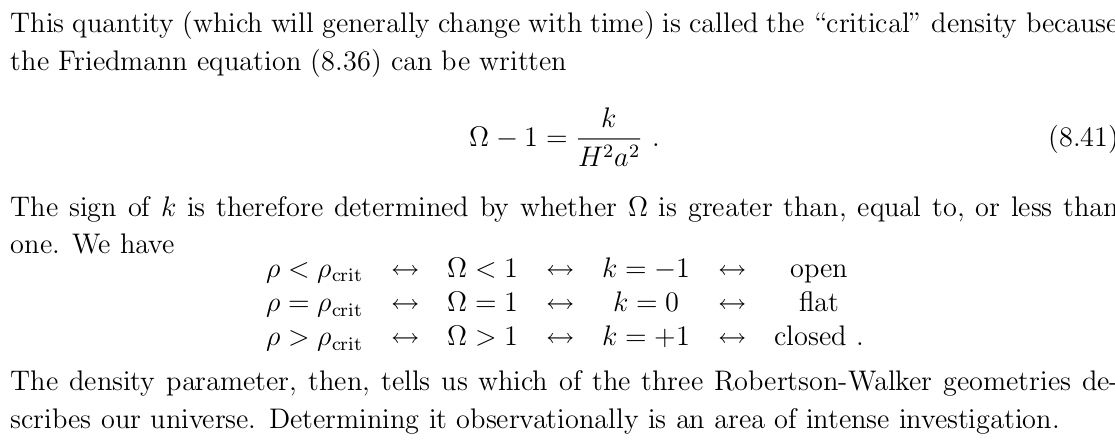
\includegraphics[width=0.7\linewidth]{gfx/criticaldensityCosomology}
	\caption{}
	\label{fig:criticaldensitycosomology}
\end{figure}

\subsubsection{On Killing Vectors in FLRW}
To understand how these quantities might conceivably be measured, let’s consider geodesic motion in an FLRW universe. There are a number of spacelike Killing vectors, but no timelike Killing vector to give us a notion of conserved energy. There is, however, a Killing
tensor. If $U^μ = (1, 0, 0, 0)$ is the four-velocity of comoving observers, then the tensor
\begin{equation} 
K\munu = a^2 (g\munu + U_μ U_ν )
\end{equation}
satisfies $∇_{(σ} K_{μν)} = 0$, and is therefore a \emph{Killing tensor}.Just as a Killing vector implies a constant of geodesic motion, if there exists
a Killing tensor then along a geodesic we will have
\begin{equation}
K_{\mu_1 \dots \mu_n} \frac{\md x^{\mu_1}}{\md \lambda } \dots \frac{\md x^{\mu_n}}{\md \lambda}=const.
\end{equation}
This means that
if a particle has four-velocity $V^μ = dx^μ /dλ$, the quantity
\begin{equation}
K^2= K\munu V^\mu V^\nu = a^2 \left[V^\mu V_\mu + (U_\mu V^\mu)^2\right]
\end{equation}
will be a constant along geodesics. Let’s think about this, first for massive particles. Then
we will have $V^μ V_μ = −1$, or
\begin{equation}
(V_0)^2 = 1 + g_{ij}V^i V^j = 1 + \abs{\vec{V}}^2.
\end{equation}
The Killing tensor then implies
\begin{equation}
\abs{\vec{V}} = \frac{K}{a}.
\end{equation}
The particle therefore “slows down” with respect to the comoving coordinates as the universe
expands. In fact this is an actual slowing down, in the sense that a gas of particles with
initially high relative velocities will cool down as the universe expands.\\
similar thing happens to null geodesics. In this case $V^2 = 0$, and $K^2=...$ implies
\begin{equation}
U_\mu V^\mu = \frac{K}{a}.
\end{equation}
But the frequency of the photon as measured by a comoving observer is $ω = −U^μ V_μ$ . The
frequency of the photon emitted with frequency $ω_1$ will therefore be observed with a lower
frequency $ω_0$ as the universe expands
\begin{equation}
\frac{\omega_1}{\omega_0} = \frac{a_0}{a_1}
\end{equation}
Cosmologists like to speak of this in terms of the redshift $z$ between the two events, defined
by the fractional change in wavelength:
\begin{equation}
z=\frac{\lambda_0-\lambda_1}{\lambda_1} = \frac{a_0}{a_1}-1.
\end{equation}
Notice that this redshift is not the same as the conventional Doppler effect; it is the expansion
of space, not the relative velocities of the observer and emitter, which leads to the redshift. But they´re are indistinguishable by Bartelmann, c.f. Cosmology section later. \todo{LOOK AT CAROLL PAGE 229 FOR INTERESTING DISTANCE MEASUREMENT TREATMENT IN COSMOLOGY SECTION}







\subsection{Comoving Coordinates Weinberg}
Imagine a finite region of space filled with a sen

\todo{Go through Comoving Coodinates on p338 by Weinberg to get a better notion of comoving coordinates and seperate its meaning from Rieamnnian normal coordiantes}



\subsection{Cosmological redshift- TO DO}
Assume both source and observer are comoving with the cosmic flow. Note that the adapted coordinates introduced before are the usual comoving coordinates :	



\newpage

\section{Friedmann models - A physical approach -- streamline with the above}
\subsection{Symmetry assumptions and consequences}
Cosmology rests on two fundamental assumptions
\begin{enumerate}
	\item When averaged over sufficiently large scales \footnote{Approximately $>200$Mpc.}, the observable properties of the universe are isotropic, i.e. independent of direction.
	\item Cosmological principles: Our position in the universe is by no means preferred to any other. The universe is spatially homogeneous.
\end{enumerate}
If the universe is isotropic around all of its points, it is also homogeneous.\\
Another assumption is that cosmology is described by general relativity. There, spacetime is a four-dimensional manifold whose metric tensor $g\munu$ is a dynamical field.\\
Rephrase the assumptions:
\begin{enumerate}
	\item 	When averaged over sufficiently large scales, there exists a mean motion of matter and energy in the universe with respect to which all observable properties are isotropic.\footnote{This is basically the comoving frame. I.e. the assumption says that there always exists a mean motion (i.e. a frame) under which spacetime appears to be isotropic.}
	\item All \textbf{fundamental observers}, i.e. imagined observers following this mean motion, experience the same history of the universe, i.e. the same averaged observable properties, provided they set their clocks suitably.	
\end{enumerate}
These assumptions translate into assumptions onto the metric of the underlying spacetime
\begin{enumerate}
	\item Time synchronization criterion \begin{equation}
		\abs{\md s}= c\md t,\quad g_{00} = - c^2.
	\end{equation}
	\item Required due to isotropy
	\begin{equation}
		g_{0i} = 0,\quad +\quad \abs{\md s}=c \md t.
	\end{equation}
	\item Because spacetime can be decomposed into spatial hypersurfaces of constant time, they can be scaled by a scale factor $a(t)$. I.e., the spacetime is described by the Robertson-Walker metric for a homogeneous and isotropic spacetime \ref{eq:metricRobertsonWalkerViaField}:
	\begin{align}
		\md s^2 &= g\munu \md x^\mu \md x^\nu = -c^2 \md t^2+a^2(t) \md l^2 \nonumber \\
		\md s^2 &= -c^2 \md t^2+ a^2(t) \left[\md w^2 + f^2_K(w) \md \Omega^2\right]
	\end{align}
Note here that $\md t$ is coordinate time, not the proper time. Further, with the normalization $a(t_0)=1$ we have that $\md l$ measures comoving distance, which is formally given by
\begin{equation}
\label{eq:conformaldistance}
	a \md \eta = - a \md \chi \quad \Rightarrow \; \chi = c \int_a^1 \frac{\md \tilde{a}}{\tilde{a}^2H(\tilde{a})},
\end{equation}
where $\eta$ is the \emph{conformal time}
\begin{equation}
	\label{eq:conformaltime}
	\md \eta = \frac{\md t}{a(t)}.
\end{equation}
\item Isotropy requires three-space to have spherical symmetry
\begin{equation}
	\md l^2 = \md w^2 + f^2_K(w) \left[\md \theta^2 + \sin^2 \theta \md \phi^2\right].
\end{equation}
\item Homogeneity requires
\begin{equation}
	f_K(w)= \left\{	\begin{array}{lll}
K^{-\half} \sin(\sqrt{K}w) & K>0 \\
w & K=0\\
\abs{K}^{-\half} \sinh(\sqrt{\abs{K}} w) & K<0\\
	\end{array}	\right\}
\end{equation}
with $K$ a constant ($[K]=cm^{-2}$) which parametrizes the curvature of spatial hypersurfaces.
\end{enumerate}
\subsubsection{Hubble law}
Note that we can expand the scale factor in a power series
\begin{equation}
	a(t_1) = a(t_0) \left[1+(t_1-t_0)H_0+\dots\right]
\end{equation}
which gives us the Hubble law for $z\ll 1$:
\begin{equation}
	z=H_0 (t_0-t_1)+\dots
\end{equation}
\subsection{Friedmann equations}
Einstein's field equations reduce to two DGL's for the scale factor $a(t)$, one equation from the time-time part and one from the three equal space-space parts of the field equations. The space-time and time-space part vanished due to our assumptions. 
\begin{mybox}{The first Friedmann equation}
	The first Fridmann equation reads
	\begin{align}
		\label{eq:friedmanneq1}
		\left(\frac{\dot{a}}{a}\right)^2 &= \frac{8 \pi \mG}{3 }\rho - \frac{K c^2}{a^2} + \frac{\Lambda c^2}{3} \nonumber \\
		\Leftrightarrow \quad H^2(t) &= H^2_0 \left[\Omega_{r,0} a^{-4} + \Omega_{m,0} a^{-3} + \Omega_{\Lambda,0} + \Omega_K a^{-2}\right]\nonumber \\
		&\equiv H^2_0 E^2.
	\end{align}
Note how all  density contributions in square brackets scale with different powers of $a$. Their relative importance thus changes over time. Today, the radiation density is much smaller than the matter density. Before a time $t_{eq}$ with
\begin{equation}
	a(t_{eq}) =: a_{eq} = \frac{\Omega_{r,0}}{\Omega_{m,0}}
\end{equation}
the universe is called \emph{radiation dominated}, $a_{eq} = 1.95 \cdot 10^{-4}$.
\end{mybox}
\begin{mybox}{Second Friedmann equation}
	\begin{align}
		\label{eq:friedmanneq2}
		\frac{\ddot{a}}{a} & = - \frac{4 \pi \mG}{3} (\rho + \frac{3 p}{c^2}) + \frac{\Lambda c^2}{3} \\
		&= H^2 +\dot{H} = - \half H^2_0 \left[\Omega_{m,0}a^{-3}-2 \Omega_{\Lambda,0}\right] \nonumber.
	\end{align}
A metric with a scale factor that satisfies \ref{eq:friedmanneq1},\ref{eq:friedmanneq2} is called \emph{Friedmann-Lemaitre-Robertson-Walker metric}.
\end{mybox}
\begin{mybox}{Adiabatic equation}
	\ref{eq:friedmanneq1} and \ref{eq:friedmanneq2} can be combined into the \emph{adiabatic equation} or the first law of thermodynamics without heat ($\delta Q=0$)
\begin{equation}
\frac{\md}{\md t}\overbrace{( a^3 \underbrace{\rho c^2}_{\epsilon})}^{\text{internal energy in volume }V=U} + p \frac{\md}{\md t}(\underbrace{a^3}_{V}) = 0,
\end{equation}
where $\rho,a,p$ are all functions of $t$. This equation intuitively states energy conservation:\\
The LHS is the change in internal energy, the RHS is the pressure work. The heat flow is absent because it would violate isotropy.
\end{mybox}



\subsection{Parameters}
\subsubsection{Pressure, density and equation of state}
With the energy density $\epsilon$ and the \emph{equation of state parameter} $\omega$, we can define the \emph{equation of state}
\begin{equation}
	p(t) = \omega \epsilon = \omega \rho(t) c^2,\quad \omega= \left\{		\begin{array}{lll}
\frac{1}{3} & \text{ ultra-rel. matter, i.e. fermion and bosonic}\\
0 &\text{non-rel. matter, thermal pressure is negligible}\\
-1 &\text{cosmic inflation, comoslogical constant, dark energy, vacuum}\\
	\end{array}	
	\right\}
\end{equation}
The pressure terms adds to the density because pressure is a consequence of particle motion, i.e. the kinetic energy of particles, which is equivalent to a mass density and thus acts gravitationally 
.\footnote{Cosmological constant can be interpreted as a type of matter, whose pressure is equal to its negative energy density.}
\footnote{Relativistic matter is what one calls radiation in cosmology and non-rel. matter is called dust.}
The adiabatic equation yields the density dependence on the scale factor:
\begin{equation}
	\rho(t)=\rho(t_0) a(t)^{-3(1+\omega)}.
\end{equation}
Consider the following equation of state parameters
\begin{enumerate}
	\item For non-rel. matter, $\omega=0$:\\
	\begin{equation}
		\rho_m(t)=\rho_{m,0}a^{-3}(t).
	\end{equation}
The density of non-rel. matter is decreasing because of dilution as space is expanding.
\item For radiation, $\omega=\frac{1}{3}$:\\
\begin{equation}
	\rho_r(t)=\rho_{r,0} a^{-4}(t),\qquad \lambda \propto a.
\end{equation}
The density of ultra-relativistic particles drops faster by one more power of $a$ because particles are diluted as space is expanding and lose energy as they are redshifted.
\item For dark energy, $\omega=-1$:\\
\begin{equation}
\rho \propto a^0.
\end{equation}
\end{enumerate}


\subsubsection{Density parameters and parameter values}
The density parameter $\Omega$ is defined as the ratio of the actual (or observed) density $\rho$ to the critical density $\rho_{cr}$ of the Friedmann universe. Then, $\rho_{cr}(t)$ is the critical density for which the spatial geometry is flat (or Euclidean).\\
\begin{mybox}{Density parameters}
With the critical density today $\rho_{cr,0}=1.86\times 10^{-29} h^2 g cm^{-3}$ corresponding to a galaxy mass per $Mpc^3$, we get
\begin{align}
	\Omega_r(t)&= \frac{\rho_{r,0}}{\rho_{cr}} a^{-4}(t)=\Omega_{r,0}a^{-4}(t),\\
	\Omega_m(t)&= = \frac{\rho_{m,0}}{\rho_{cr}} a^{-3}(t) = \Omega_{m,0} a^{-3}(t) \\
	\Omega_{\Lambda} (t) &= \frac{\Lambda c^2}{3 H^2(t)}\quad \text{with} \\
	\rho_{cr}(t)&= \frac{3 H^2(t)}{8 \pi \mG} \\
	\Omega_K &:= 1-\Omega_{r}-\Omega_{m}-\Omega_{\Lambda}= - \frac{K c^2}{H^2}.
\end{align}
\end{mybox}
Note that we therefore have
\begin{align}
	\rho_r(a)&= \Omega_{r,0} \rho_{cr,0} a^{-4},\\
	\rho_m(a) &= \Omega_{m,0} \rho_{cr,0} a^{-3}\\
	\Omega_r(a) &= \frac{\Omega_{r,0} a^{-4}}{E^2(a)}\\
	\Omega_{m}(a) &= \frac{\Omega_{m,0} a^{-3}}{E^2(a)}.
\end{align}
Two comments are in order:
\begin{enumerate}
	\item If $\Omega_{K,0} \approx 0$ today, then it is even more negligible going back in time, as $\Omega_r,\Omega_m$ dominate past $\Omega_K$ by far.
	\item What does $\rho_{cr}(t)$ represent ? We can bring it into the following form:
	\begin{equation}
		\rho_cr(t) = \dots \; \Leftrightarrow \; \frac{4 \pi \mG}{3} \left(\frac{\rho_{cr} a^3}{a}\right) = \frac{\dot{a}^2}{2}.
	\end{equation}
	From this we can read off the following interpretation: ’A sphere whose matter is completely filled with critical density has the property, that its kinetic energy exactly equals out the potential energy per particle.’
\end{enumerate}
\begin{mybox}{Hubble parameter}
	The \emph{Hubble parameter} is defined as the relative expansion rate 
	\begin{equation}
	\label{eq:hubbleparameter}
	H(t):= \frac{\ddot{a}(t)}{a(t)}
	\end{equation}
	with the \emph{Hubble constant}
	\begin{equation}
		\label{eq:hubbleconstant}
		H(t_0)=: H_0 = 100 h \;\frac{km}{s Mpc} = 3.22\times 10^{-18} h \; s^{-1}.
	\end{equation}
	It quantifies by how much the \emph{recession velocity} of cosmic objects grows as their distance increases. \textbf{Every length scale changes by $H_0$ per second}.
\end{mybox}
The \emph{Hubble time} is
\begin{equation}
	t_H = \frac{1}{H_0} = 9.82 \times 10^9 \frac{yr}{h} \approx 15 Gyr.
\end{equation}
The \emph{Hubble radius} is
\begin{equation}
	r_H=\frac{c}{H_0} = 3.01 \times 10^3 \frac{Mpc}{h} \approx 5 Gpc.
\end{equation}
\begin{mybox}{Evolution of epochs}
	 \begin{tabular}{|l|llll|}
		          & $\omega$ & $\rho(a)$ & $a(t)$ & $a(\tau)$ \\
		\toprule
		\text{radiation dominated, RD} & $\frac{1}{3}$&$a^{-4}$&$t^{\half}$ & $\tau$ \\
		\text{Matter dominated, MD} & $0$ & $a^{-3}$ & $t^{\frac{2}{3}}$ & $\tau^2$ \\
		$\Lambda$\text{ dominated, $\Lambda$D} & $-1$ & $a^0$ & $e^{H_0 \sqrt{\Omega_{\Lambda,0} t} }$ &$-\tau^{-1}$\\
		\bottomrule
	\end{tabular}
\end{mybox}
\begin{figure}[h!]
	\centering
	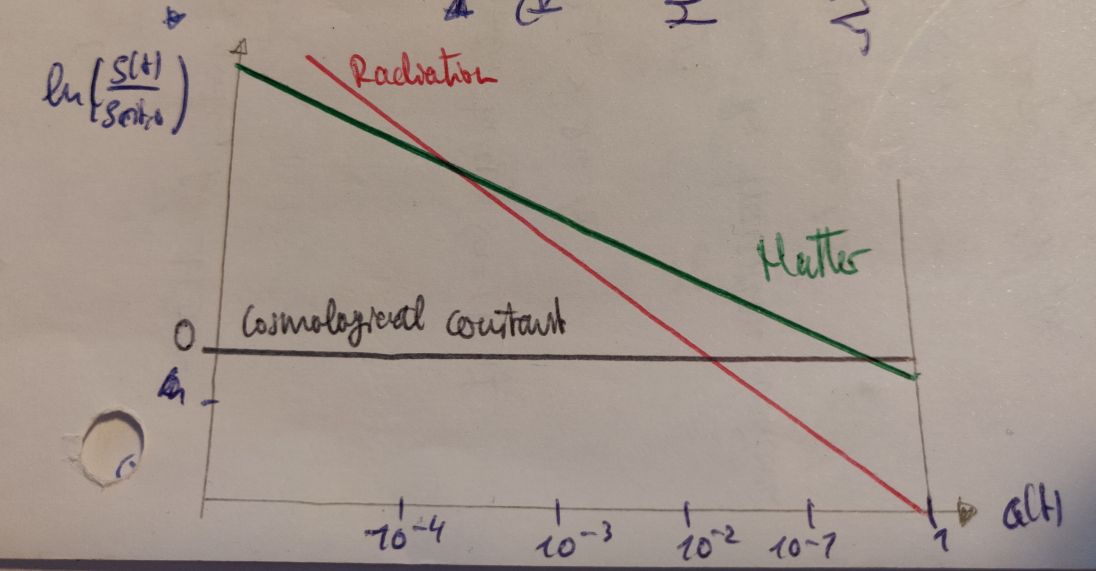
\includegraphics[width=0.7\linewidth]{gfx/EvolutionEpochs}
	\caption{}
	\label{fig:evolutionepochs}
\end{figure}
\subsection{Redshift (cosmological)}
\subsubsection{Role of the observer - Definitions}
\begin{mybox}{Comoving observer}
	A \emph{comoving observer} is the only observer that will perceive the universe (e.g. CMB) as isotropic. Non-comoving observers will see regions of the sky systematically blue-or redshifted.\\
	Thus, isotropy in particular defines (especially isotropy of the CMB) a special local frame of reference called the \emph{comoving frame}.  \emph{Cosmic time} is then the time in the comoving frame.
\end{mybox}
\begin{mybox}{Comoving frame - coordinate system}
	Comoving coordinates assign constant spatial coordinate values to observers who perceive the universe as isotropic, hence comoving observers. We are considering the dynamics of particles
	on an expanding spatial background, the physical distance $\vec{r}$ between any two particles
	therefore grows with time in proportion to the scale factor $a ( t )$ , i.e. comoving coordinates $q$ are defined via the spatial coordinates as
	\begin{equation}
		\label{eq:comovingcoordinates}
		\vec{r}(t) = a(t) \vec{q}.
	\end{equation}
\end{mybox}
\begin{mybox}{Velocities}
	The velocity of an observer relative to the local comoving frame is called \emph{peculiar velocity} of the observer. It therefore is the component of an e.g. galaxy' s velocity that deviates from the \emph{Hubble flow} (i.e. \emph{the motion solely due to the expansion of space}). \\
	\emph{Recession velocity} is then the rate at which an astronomical object is moving away (e.g. from Earth).
\end{mybox}

\subsubsection{Redshift definition}
\begin{mybox}{Redshift}
Spatial hypersurfaces can expand or shrink by the scale factor $a(t)$. This leads to a red- of blueshift of photons propagating through spacetime
\begin{equation}
	\ref{eq:redshiftCosmo}
	\frac{a(t_{\text{observed}})}{a(t_{\text{emitted}})} \stackrel{ a(t_0)\stackrel{!}{=}1}{=} \frac{1}{a(t_e)} = 1+z = \frac{\lambda_0}{\lambda_e} = \frac{\nu_e}{\nu_0},\quad a(t_e)\equiv a.
\end{equation}\end{mybox}
Comments:
\begin{enumerate} 
	\item Derivation of the above:
This stems from the fact that for light we have
\begin{equation}
	\md s^2 =0 =-c^2 \md t^2+a^2 \md \omega^2\; \Leftrightarrow \; c\abs{\md t} = a(t) \md \omega,
\end{equation}
as light has a vanishing proper time. Now consider light emitted from a comoving source at time $t_e$ reaching a comoving observer at $\omega=0$ at time $t_o$; hence the coordinate distance between the source and observer is
\begin{equation*}
\omega_{e,o} = \int_{t_e}^{t_o} \md \omega = \int_{t_e}^{t_o}  \frac{c \md t}{a(t)} = const.
\end{equation*}
as the source and observer are both comoving. Then
\begin{equation*}
0 \stackrel{!}{=} \frac{\md \omega_{e,o}}{\md t} \; \Rightarrow \; \frac{\md t_o}{\md t_e} = \frac{a(t_o)}{a(t_e)} \Leftrightarrow \; \tau_e=\tau_o.
\end{equation*}
\item 
\end{enumerate}
\subsubsection{Big Bang}
The \emph{relative acceleration} $\frac{\ddot{a}}{a}$ is given, for $\Lambda$CDM Universe and pressure-less matter, as
\begin{equation}
\frac{\ddot{a}}{a} = H^2_0 \left[\Omega_{\Lambda,0}-\frac{\Omega_{m,0}}{2 a^3}\right].
\end{equation}
The expansion of the universe therefore accelerates today ($a=1$) if
\begin{equation}
\ddot{a} = H^2_0 \left[\Omega_{\Lambda,0}-\frac{\Omega_{m,0}}{2}\right]>0 \text{ or if } \Omega_{\Lambda,0} > \frac{\Omega_{m,0}}{2}.
\end{equation}
The latter if-statement is rendered true by measurements. Thus, \textbf{the Universe's expansion accelerates today}.\\
If the Universe indeed is spatially flat, then the transition between decelerated and accelerated expansion happened at
\begin{equation}
	1-0.263 \approx \frac{0.263}{2 a^3} \Rightarrow a = 0.56, \; z=0.78.
\end{equation}
Luminosity distances to supernovae at larger redshifts show this transition.
\subsection{Age and Expansion of the Universe}
The age of the universe can be calculated by 
\begin{equation}
	t= \int_{a(z_1)}^{a(z_2)} \frac{\md a^\prime}{a^\prime H(a^\prime)} = \frac{1}{H_0} \int_{a(z_1)}^{a(z_2)} \frac{\md a^\prime}{a^\prime E(a^\prime)}, \quad z_1>z_2
\end{equation}
setting $a(z_1)=0, a(z_2)=a$. This integral can only be solved analytically via approximations/assumptions:
\begin{enumerate}
	\item For a flat, single component universe (where the e.o.s. parameter does \emph{not} change over time), the Friedmann eq. reduces to
	\begin{equation*}
		H = H_0 \sqrt{\Omega_{I,0}} a^{-\frac{3}{2} (1+\omega_I)},
	\end{equation*}
	thus
	\begin{equation}
	a(t) \propto \left\{ \begin{array}{lll}
	t^{\frac{2}{3}(1+\omega_I)} & w_I\neq -1,&a(t)\propto \begin{array}{ll}
	t^{\frac{2}{3}} & \text{MD} \\
	t^\half & \text{RD}\\
	\end{array}		\\
	e^{H_0 \sqrt{\Omega_I} t} & \omega=-1 & \Lambda\mathrm{D}.	\end{array}\right\}
	\end{equation}
\item Einstein-deSitter: $\Omega_{r,0}=\Omega_{\Lambda,0}=0$,$\Omega_{m,0}=1,\Omega_{K,0}=0$ $\Rightarrow E(a) \approx \sqrt{\Omega_{m,0}} a^{-\frac{3}{2}}$
\begin{equation}
	t = \frac{2}{3} \frac{a^{\frac{3}{2}}}{H_0} \; \Rightarrow \; t_0 = \frac{2}{3 H_0}, \; \Leftrightarrow \; a=\left[\frac{3}{2} H_0 t\right]^{\frac{2}{3}} \propto t^{\frac{2}{3}}.
\end{equation}
This describes the universe well for $z\in [2,300]$.
\item Early Universe:
\begin{equation*}
	E(a) \approx \sqrt{\Omega_{r,0} a^{-4}+\Omega_{m,0} a^{-3}},
\end{equation*}
\begin{equation}
	\Rightarrow \; t(a=a_{eq}) = t_{eq} = \frac{2 a^{\frac{3}{2}}_{eq} }{3 H_0 \sqrt{\Omega_{m,0}}} (2-\sqrt{2}) \approx 20.000 yr \rightarrow \footnote{including neutrino partake in $\Omega_{r,0}$} 50.000 yr.
\end{equation}
The radiation dominated epoch is thus very short compared to the age of the universe. Therefore, for the most part of the cosmic time, radiation is negligible because the period of radiation domination is very brief in comparison.
\item Very later universe: $E(a)\approx \sqrt{\Omega_{\Lambda,0}}$
\begin{equation}
	\Rightarrow \quad t = \frac{\ln(a)}{H_0 \sqrt{\Omega_{\Lambda,0}}} \; \Rightarrow \; a \propto \exp\left[\sqrt{\Omega_{\Lambda,0}} H_0 t\right].
\end{equation}
Here the universe expands forever exponentially (\emph{deSitter limit}). A universe expanding with $H_0$ today may never reach $a=0$ going back in time. The fact that the universe is expanding today does thus not imply that it originated in a Big Bang. There must have been a Big Bang though, because:
\begin{enumerate}
	\item From existence of the CMB we know that radiation density is finite.
	\item From the existence of luminous material that the matter density is finite.
	\item From existence of objects with $z\gg 0$ we know that $a(z)$ must have been as small as $\frac{1}{1+z}$ or smaller in the past.
\end{enumerate}
\item ODM: $K\neq =,\Omega_{m,0} \neq 0, \Omega_{\Lambda,0}=0$.
\end{enumerate}

\subsection{Distance measures}
In general, $z$ is the only observable in cosmology (via comparison of absorption/emission lines e.g.). All distances are therefore expressed in terms of the redshift.\\
An object at higher redshift $z_2$ is more distant to us than one at $z_1 < z_2$. The more distant a source is from us, the longer the light takes to reach us, the earlier it was emitted, the smaller $a$ was at emission, ant the larger $z$ is.
\subsubsection{Proper distance - not observable}
The distance measured by the time required for light to travel from a source to an observer
\begin{mybox}{Proper distance}
	\begin{equation}
		\md D_{prop} =-c \md t,\; \Rightarrow\;	D_{prop}(z_1,z_2)= \frac{c}{H_0} \int_{a(z_2)}^{a(z_1)} \frac{\md a}{a E(a)},
	\end{equation}
	thus the distance increases as we move away from observer (therefore minus sign).
\end{mybox}
This distance changes in time and therefore has to be done about two points $z_1,z_2$ with the same cosmological time. $D_{prop}$ is what a measurement at constant cosmic time would yield.
\subsubsection{Comoving distance - not observable}
The distance on the spatial hypersurface at $t=const.$ between the world lines of a source comoving with the mean cosmic flow, thus the comoving distance accounts for the expansion of the universe. $D_{com}$ is obtained by integrating the proper distance of nearby fundamental observers along the line of sight.
\begin{mybox}{comoving distance}
	For objects moving (only) with the Hubble flow, it is deemed to remain constant in time
	\begin{equation}
		D_{com}(z_1,z_2) = \int_{a(z_2)}^{a(z_1)} \md \omega= \frac{c}{H_0} \int_{a(z_1)}^{a(z_2)} \frac{\md a}{a^2 E(a)} =: \omega(z_1,z_2).
	\end{equation}
	Another form for photons in particular (i.e. $\md s=0$, $a \md\omega=-c \md t$) $t_e$ the time of emission of photons detected by the observer and $t$ is present
	\begin{equation}
	\omega=	c \int_{t_e}^t \frac{\md t^\prime}{a(t^\prime)}.
	\end{equation}
\end{mybox}
This is the distance one acquires for solely moving with the Hubble flow. Thus dividing by $a$ scales back to initial distance, which will be constant if observer and emitter are both only moving with the Hubble flow.

\begin{figure}[h!]
	\centering
	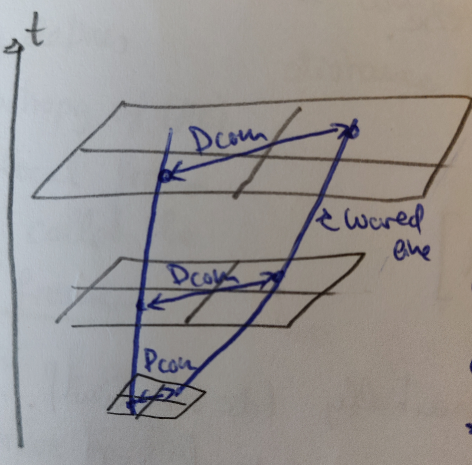
\includegraphics[width=0.7\linewidth]{gfx/comovingdistance}
	\caption{}
	\label{fig:comovingdistance}
\end{figure}





\subsubsection{Angular diameter distance}
If you know the are of the observed source $\delta A$ and measure the solid angle $\delta \Omega$ under which it appears, then you get the distance from the source to an observer via the comoving distance
\begin{equation}
	D_{ang}(z_1,z_2) = \sqrt{\frac{\delta A}{\delta \Omega}} = \frac{a(z_2)}{a(z_1)} f_K\left[D_{com}(z_1,z_2)\right].
\end{equation}
$D_{ang}$ is measured on the backward lightcone. The backward lightcone itself shrinks due to the expansion of space. Therefore, the angular size of an object changes non-monotonic w.r.t. the distance. This is due to the four-dimensional curvature of spacetime, which resolves in a focussing effect on most distance source. We therefore perceive them as being near us (by means of angular diameter distance).

\begin{figure}[h!]
	\centering
	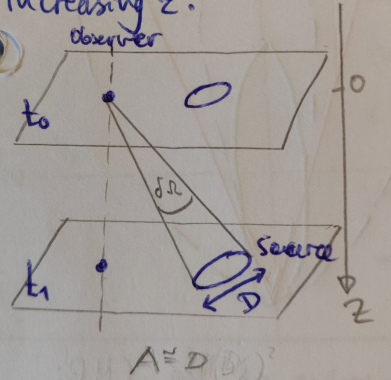
\includegraphics[width=0.7\linewidth]{gfx/AngulardiameterDistance}
	\caption{}
	\label{fig:angulardiameterdistance}
\end{figure}





$D_{ang}$ has maximum at $z=\frac{5}{4}$ in Einstein-deSitter universe and gently decreases for increasing $z$.

\begin{figure}[h!]
	\centering
	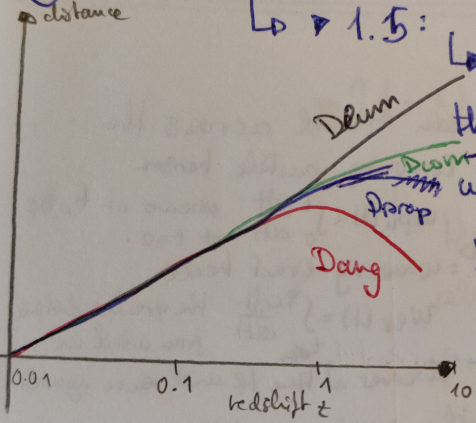
\includegraphics[width=0.7\linewidth]{gfx/DistancemeasuresCompared}
	\caption{}
	\label{fig:distancemeasurescompared}
\end{figure}

\subsubsection{Luminosity distance and Etherington relation}


\begin{figure}[h!]
	\centering
	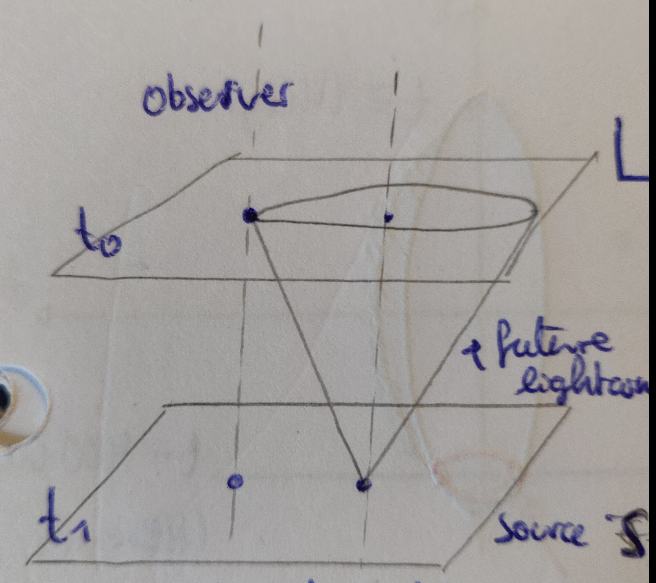
\includegraphics[width=0.7\linewidth]{gfx/AngulardiameterDistance1}
	\caption{}
	\label{fig:lumininositydistance1}
\end{figure}
For a source with bolometric luminosity $L$ and flux $S$ (i.e. at the source we have $S=\frac{L}{4 \pi d^2}$)
\begin{equation}
	D_{lum}(z_1,z_2) = \sqrt{\frac{L}{4 \pi S}}.
\end{equation}
\begin{mybox}{Etherington relation}
\begin{equation}
	D_{lum}(z_1,z_2) = \left[\frac{a(z_1)}{a(z_2)}\right]^2 D_{ang}(z_1,z_2) = (1+z)^2 D_{ang},
\end{equation}
where the latter equality holds for $z_1=0$ for observer (usually true as we mostly have measurements in the present time on Earth) and $z_2=z$ for emission/source.
\end{mybox}
Photons are therefore redshifted by $\frac{a_1}{a_2} >1$ between emission and absorption, their arrival times are strecthed by $\frac{a_1}{a_2}$ and they are spatially diluted by factor $\left(\frac{a_1}{a_2}\right)^2$, thus $L\propto \left(\frac{a_1}{a_2}\right)^4 S$. Therefore, the Etherington relation gives the scale factor between the shrinking backward lightcone and forward lightcone.
\\
\\
To recapitulate, the Angular diameter distance is a measurement on the backward lightcone (compare \ref{fig:angulardiameterdistance}). The luminosity distance is exactly the opposite (compare \ref{fig:lumininositydistance1}). The flux is the section we receive from the source, compare \ref{fig:luminositydistance}.
\begin{figure}[h!]
	\centering
	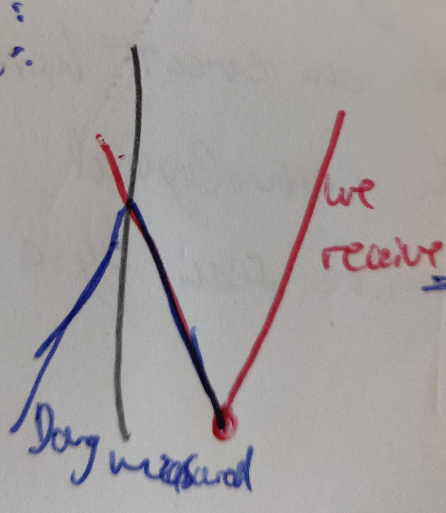
\includegraphics[width=0.7\linewidth]{gfx/luminositydistance}
	\caption{}
	\label{fig:luminositydistance}
\end{figure}
\newpage
\subsection{Horizons}
Horizons occur because of the finite speed of light and the expansion of the Universe:
\begin{enumerate}
	\item There exists a \emph{particle horizon}, i.e. light can only travel by a finite distance between the Big Bang and any later time, thus any particle in the universe can only be influenced by events within a finite region.
	\item There exists an event horizon if the expansion of the universe is dominated by the cosmological constant at late times. Then, the region which can be seen by a particle remains finite.
\end{enumerate}
Formulate these horizons in explicit terms.\\
Between times $t_1$ and $t_2 > t_1$, light can travel across the comoving distance
\begin{equation}
	\Delta \omega(t_1,t_2)= \int_{t_1}^{t_2} \frac{c \md t}{a(t)} = \frac{c}{H_0} \int_{a(t_1)}^{a(t_2)} \frac{\md a^\prime}{{a^\prime}^2 E(a^\prime)}.
\end{equation}
This gives us two different kinds of horizons.
\begin{mybox}{Horizons}
	\begin{enumerate} 
		\item 
	\emph{Comoving particle horizon}
	\begin{equation}
		\omega_{ph}(t)=\int_0^t \frac{c \md t}{a(t)}
	\end{equation}
	with observer at $t$ and Big Bang at $t=0$.
	\item \emph{Comoving event horizon}
	\begin{equation}
		\omega_{eh} (t) = \int_t^{t_f} \frac{c \md t}{a(t) }
	\end{equation}
	which is the greatest possible distance from which an observer at time $t_f$ will receive signals.
\end{enumerate}
\textbf{Altogether, the region that we perceive (particle horizon) is finite and the region we can influence (event horizon) is finite}.
\end{mybox}
\textbf{Our backward lightcone is all of the universe we can see, a tiny fraction of the actual universe.}
\begin{figure}[h!]
	\centering
	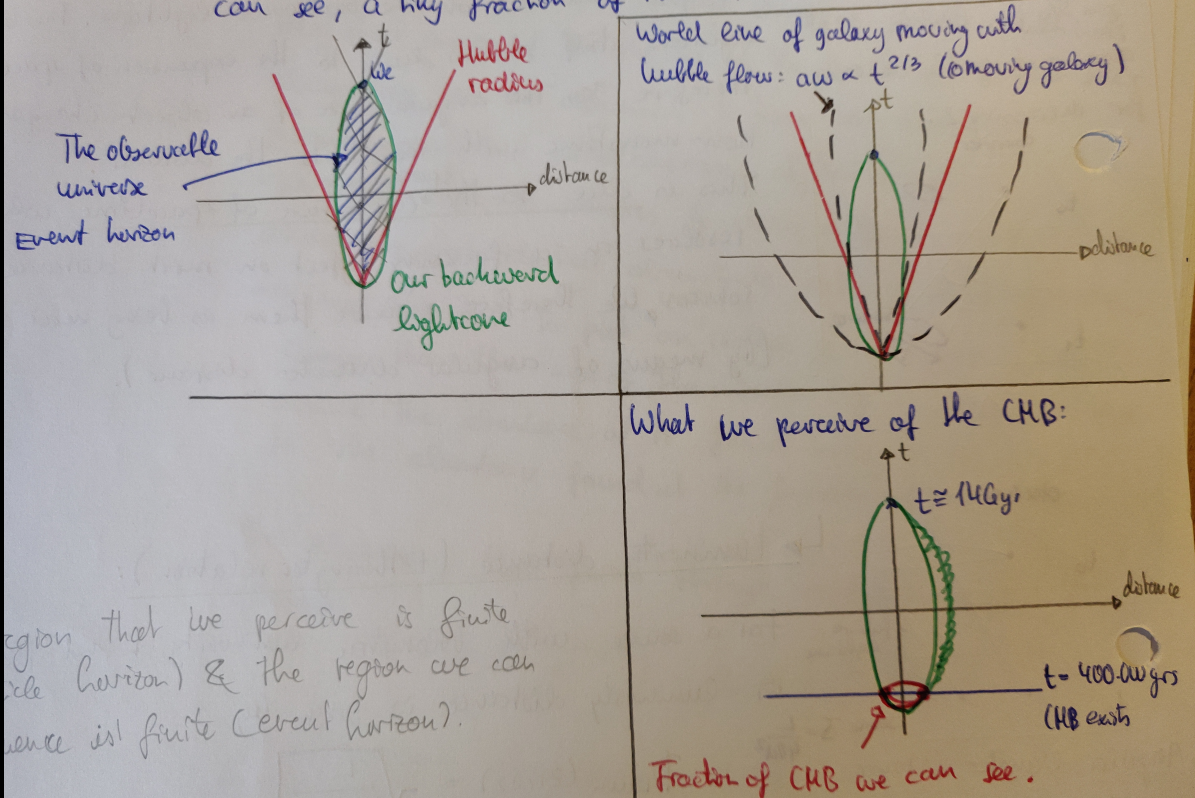
\includegraphics[width=0.7\linewidth]{gfx/Horizons}
	\caption{}
	\label{fig:horizons}
\end{figure}


















\section{Age of the Universe and the cosmic expansion}
\subsection{Nuclear cosmo-chronology}
\subsection{Stellar ages}
\subsection{Cooling of white dwarfs}
\subsection{The Hubble constant}
\subsection{Supernovae of type Ia}




\section{Thermal evolution of the universe}
\subsection{Assumptions and quantum statistics}
\subsubsection{Assumptions}
The underlying assumptions are
\begin{enumerate}
\item \emph{The universe expands adiabatically}-\\
isotropy requires the universe expand adiathermally: no heat can flow because flow directions would violate isotropy. Adiathermal expansion is adiabatic if it is reversible, thus if entropy does not change. Entropy does indeed changed, but, because of $\frac{n_{\text{Baryon}}}{n_\gamma} \approx 10^{-9}$, the entropy from electromagnetic radiation of the CMB dominates the entropy of the universe by far $\Rightarrow$ entropy generations completely negligible.
\item \emph{Thermal equilibrium can be maintained despite the expansion} $\Leftrightarrow$ At very early times, there was thermal equilibrium between interacting particle species-\\
thermal equilibrium can only be maintained if the interaction rate of particles is higher than the expansion rate of the Universe. For $t\rightarrow0$, particle densities grow so fast that interaction rates are indeed higher than the high expansion rates at early times. As the universe proceeds to expand, now and then then single particle species will fall out of thermal equilibrium.\\
\\ From the perfect black-body spectrum of the CMB we have good observational evidence that the early universe was in local thermal equilibrium. This perfect planck black-body spectrum also implies that the universe was in thermal equilibrium during decoupling and even so later on. Particles maintain thermal equilibrium due to direct collisions (Thomson scattering). The thermal equilibrium disappears, because energies of particles and scattering cross sections become very low. This is because the mean free path becomes very large, i.e. interactions/collisions are not very likely to happen.
\item \emph{The cosmic ’fluids’ can be treated as ideal gases}- \\
thus there are no long-range interactions between particles, they can only interact by direct collisions. Holds also for charged particles, because oppositely charged particles shield each other.\footnote{Note that for charged particles, the Couloum-potential goes like Yukawa-potential, i.e. has an exponential cut-off. Therefore, this is a valid approximation.}
\end{enumerate}

\subsubsection{Recap on quantum statistics}
\begin{enumerate}
	\item The ensemble is \emph{canonical}, if the mean internal energy is specified. I.e. Helmholtz free energy
	\begin{equation}
		F=-k_B T \ln(Z_c),\quad Z_c=\sum_\alpha \exp[-\frac{\epsilon_\alpha}{k_B T}]
	\end{equation}
	with $Z_c$ the canonical partition sum over all accessible quantum states.
	\item The ensemble is \emph{grand-canonical}, if only the mean number of particles is specified. This transitions to the grand-canonical potential
	\begin{equation}
		\mJ = - k_B T \ln(Z_{gc})
	\end{equation}
	with the gc partition sum $Z_{gc} = \prod_\alpha Z_\alpha$ with
	\begin{equation}
		Z_\alpha = \sum_{N_\alpha} e^{-(\epsilon_\alpha-\mu) \frac{N_\alpha}{k_B T}} = \left\{	\begin{array}{ll}
	1+e^{-\frac{(\epsilon_\alpha-\mu)}{k_B T}} & \text{fermions} \\
	1-e^{-\frac{(\epsilon_\alpha-\mu)}{k_B T}} & \text{bosons} \\
		\end{array}		\right\}.
	\end{equation}
	By 
	\begin{equation}
		N_\alpha = \left\{ \begin{array}{ll}
		0,1 & \text{fermions} \\
		0,1,\dots,\infty & \text{bosons} \\
		\end{array}			\right\}
	\end{equation}
	it follows that the mean occupation number of a quantum state $\alpha$ is
	\begin{equation}
		\bar{N}_\alpha= \frac{1}{e^{\frac{\epsilon_\alpha-\mu}{k_B T}} \pm 1}, \quad \begin{array}{ll}
		+ & \text{fermions}\\
		- & \text{bosons, diverges for Bose Condensation}\\
		\end{array}.
	\end{equation}
	The spatial number density in thermal equilibrium is
	\begin{equation}
		n = \sum_\alpha N_\alpha = \int \md N = \int g \frac{V}{(2\pi)^3} \md^3 p = \int \frac{\md^3 p}{(2 \pi)^3} \frac{g}{e^{\frac{\epsilon(p)}{k_B T} }\pm 1},
	\end{equation}
	with $g$ being the statistical weight, i.e. $g_\gamma=2$ for photons and otherwise $g=2s+1$ for spin-$s$ particles, and with 
	\begin{equation}
		\epsilon(p) = \left\{\begin{array}{ll}
		cp & \text{ultra-rel. gas} \\
		\sqrt{c^2 p^2+m^2c^4} & \text{rel. gas} \\
		\frac{p^2}{2m} & \text{non-rel. gas} \\
		\end{array}		\right\}.
	\end{equation}
	Thus, the mean energy density in thermal equilibrium is
	\begin{equation}
	U = \int \pmeasure \frac{g \epsilon(p)}{e^{\frac{\epsilon(p)}{k_B T}} \pm 1 }.
	\end{equation}
\footnote{$1eV=1.6\times 10^{-12}erg$, i.e. $k_B T = 1.16\times 10^4 K$.}
	\begin{mybox}{Ultra-rel. boson in thermal equilibrium}
		\begin{align}
			N_B &= g_B \frac{\zeta(3)}{\pi^3} \left(\frac{k_B T}{\hbar c}\right)^3 \quad \propto T^3\\
			U_B &= g_B \frac{\pi^2}{30} \frac{(k_B T)^4}{(\hbar c)^3}\quad \propto T^4\\
			P_B &= \frac{1}{3} U \quad \propto T^4\\
			S_B &= g_B k_B \frac{2 \pi^2}{45} \left(\frac{k_B T}{\hbar c}\right)^3 \quad \propto T^3.
		\end{align}
	\end{mybox}
\begin{mybox}{Ultra-rel. fermions in thermal equilibrium}
	\begin{align}
		n_F &= \frac{g_F}{g_B} n_B=\frac{3}{4} n_B \quad \propto T^3\\
		u_F &= \frac{7}{8} u_B \quad \propto T^4\\
		P_F &= \frac{g_F}{g_B} P_B=\frac{7}{8} P_B \quad \propto T^4 \\
		S_F &= \frac{3}{4} S_B \quad \propto T^3.
	\end{align}
\end{mybox}
\item For non-rel. classical gas we acquire the Maxwell-Boltzmann distribution
\begin{align}
n&= \left(\frac{m k_B t}{2 \pi^2 \hbar^2}\right)^\frac{3}{2} \exp\left[-\frac{mc^2}{k_B T}\right]\\
u&=c_V n = \frac{f}{2} n k_B T,\\
P&= nk_B T.
\end{align}\footnote{By comparing the rel. limit $k_B T \gg mc^2$, we see that the number density, energy density, and pressure of a particle species fall exponentially (are "\emph{Boltzmann suppressed}") as the temperature drops below the mass of the particles.}
\end{enumerate}
Note that the \emph{chemical potential} $\mu$ encodes what it costs to move, i.e. $\partial_N U$ one particle from one place to another. The chemical potential characterizes the response of a system to a change in particle number
\begin{equation}
\label{eq:chemicalpotential}
	\mu = - T \left(\frac{\partial S}{\partial N}\right)_{U,V}.
\end{equation}
The second law of thermodynamics means that particles flow to the side of the reaction with the lower total chemical potential. Chemical equilibrium is reached when the sum of the chemical potentials of the reacting particles is equal to the sum of the chemical potentials of the products. The rates of the forward and reverse reaction are then equal.
\subsubsection{Adiabatic expansion of ideal gas}
In thermal equilibrium we have
\begin{enumerate}
	\item For rel. boson or fermion gases, we have $P=\frac{u}{3}= \frac{E}{3V}$
	\item For non-rel. gases $U = \half f N k_B T$.
\end{enumerate}
By the first law of thermodynamics in absence of heat transfer $\md E + P\md V=0$ we find
\begin{equation}
T\propto \left\{\begin{array}{ll}
V^{-\frac{1}{3}} \propto a^{-1} & \text{rel. boson or fermion gas }\gamma=\frac{4}{3} \\
V^{-\frac{5}{3}+1} \propto a^{-3(1-\gamma)} \propto a^{-2} & \begin{array}{ll}
\gamma=\frac{5}{3}&\text{non-rel 1-atomic, ideal gas } \\
\gamma=\frac{9}{7}& \text{ for diatomic molecule}\\
\end{array}
\end{array}			\right\}.
\end{equation}
Therefore the temperature of non-rel. gases drops faster with the expansion of the universe. Further on we see that the temperature of things in the universe will be maintained equally early on, but will differ more and more with expansion.\\
For non-rel. gases we have to consider the explicit degree of freedom

	 \begin{tabular}{|l|llll|}
	& $\bullet$ & $2$-atomic identical (3 transl.$+2$ rot.) & $2$-atomic non-identical ($3$ transl. $+4$ rot..) \\
	\toprule
$\gamma$ &$\frac{5}{3}$ & $\frac{7}{5}$ & $\frac{9}{7}$\\
$f$ & $3$ & $5$ & $7$ \\
	\bottomrule
\end{tabular}
thus
\begin{equation}
	T\stackrel{\stackrel{f\rightarrow\infty}{\gamma \longrightarrow 1}}{\longrightarrow} constant.
\end{equation}



\subsubsection{Particle freeze out}
At early times (radiation-dominated era) the expansion time-scale is
\begin{equation}
	t_{exp} \approx \frac{1}{\sqrt{\mG \rho}}\propto a^2.
\end{equation}
The expansion time-scale (e.g. time-scale for universe to double its radius) is very brief thus increases rapidly as the universe expands away from the Big Bang.\\
\\
Whether the assumption of thermal equilibrium is valid is shown by comparison of expansion rate of the universe to the interaction rate of particles.\\
Thermal equilibrium is maintained predominantly by two-body interactions. The collision rate is, where $n\propto T^3$ for rel. particles, 
\begin{equation}
	\Gamma:= \frac{\md N}{\md t}= n \expval{\sigma v} \propto n \propto T^3 \propto a^{-3}. 
	\end{equation}
	\footnote{In the second step we used: For a process like $1+2\leftrightarrow 3+4$ we would write the interaction rate of species $1$ as $\Gamma_1=n_2 \sigma v$, where $n_2$ is the density of the target species $2$ and $v$ is the average velocity of $1$ and $2$. The interaction rate of species $2$ would be $\Gamma_2=n_1 \sigma v$. We have used the epxectation that at high energies $n_1 \approx n_2 \equiv n$.}
This shows that different particle species may have different interaction rates and so may decouple at \textbf{different times}.\\
The collusion time scale is thus
\begin{equation}
	t_{coll} = \Gamma^{-1} \propto a^3.
\end{equation}
\begin{mybox}{Validation of thermal equilibrium assumption}
Thus
\begin{equation}
	\frac{t_{exp}}{t_{coll}} \propto a^{-1} \stackrel{a\rightarrow 0}{\longrightarrow} \infty,
\end{equation}
which implies that the collisions have a much shorter time scale than the expansion in the early universe. Thermal equilibrium can thus be maintained despite the expansion in particular at early times. As the universe keeps expanding, collisions become rare and thermal equilibrium will ultimately break down.
\end{mybox}
The continuity equation of particle numbers in the universe is regulated by the destruction through collisions (i.e. $\Gamma$) and by thermal creation ($n_T=$ thermal number density, creation due to e.g. collisions).\\
In the absence of interactions, it reads per particle species $i$
\begin{equation}
\frac{\md n_i}{\md t} + 3 \frac{\dot{a}}{a} n_i=0.
\end{equation}
\begin{mybox}{Freeze-out or Boltzmann equation}
Noting $\Gamma_1=n_2 \expval{\sigma v}$ and introducing the comoving number density $N=a^3n$, we find from this continuity equation
\begin{equation}
\frac{\md \ln N_1}{\md \ln a} = - \frac{\Gamma_1}{H(a)}\left[1 -\frac{N^2_{T,1}}{N^2_1}\right] =\begin{array}{ll}
\frac{\md \ln N}{\md \ln a}>0 & N<N_T\\
\frac{\md \ln N}{\md \ln a} <0 & N>N_T\\
\end{array},
\end{equation}
such that for $N<N_T$ there are more particles produced until $N=N_T$ whereas for $N>N_T$ particles get destroyed in order to get back to $N=N_T$.\\
Overall, no matter the initial conditions, the thermal number will be established for frequent collision rates and $N\gg0$.
\end{mybox}
\footnote{On the freeze-out equation: For $\Gamma_1\gg H$ the natural state of the system is chemical equilibrium. Imagine that we start with $N_1 \gg N_{1,T}$. The RHS then is negative, particles of type $1$ are destroyed and $N_1$ is reduced towards the equilibrium value $N_{T,1}$. Similarly, if $N_1\ll N_{1,T}$, the RHS is positive and $N_1$ is driven towards $N_{1,T}$. As long as the interaction rates are large, the system quickyl relaxes to a steady state where the RHS vanishes and the particles assume their equilibrium abundances. Thus, ’\textbf{with interaction rates high, particles retain the equilibrium state}’. When the reaction rate drops below the Hubble scale $\Gamma_1 <H$, the RHS gets suppressed and the comoving density of particles approaches a constant relic density, i.e. $N_1=$constant.}
About the freeze out equation:\\
If $N=N_T$, it does not change. If $N$ deviates from $N_T$, it needs to change for readjustment to its thermal equilibrium value $N_T$. This is not possible for $\Gamma \ll H$, because then the rate of change becomes too small. Then, the particles freeze out of thermal equilibrium.\\
\\
We find:
\begin{enumerate}
	\item For relativistic particles 
	\begin{equation*}
	n\propto T^3 \propto (a^{-1})^3 = a^{-3} \quad \Rightarrow \quad N=\text{constant}
	\end{equation*} 
	with
	\begin{equation}
		\frac{\md \ln N}{\md \ln a} =0 \quad \Rightarrow \quad N=N_T.
	\end{equation}
	This implies that relativistic particle species retain their thermal-equilibrium density regardless of $\frac{\Gamma}{H}$, i.e. even after freeze-out.
	\item For non-rel. particles 
	 \begin{equation*}
	 	N_T \propto T^{-\frac{3}{2}} \exp\left[-\frac{mc^2}{k_B T}\right].
	 \end{equation*}
	 For $k_B T\leq mc^2$, $N_T$ drops exponentially: $N_T  \ll N$
	 \begin{equation}
	 	\frac{\md \ln N}{\md \ln a} \approx -\frac{\Gamma}{H} \rightarrow 0
	 \end{equation}
	 as the collision rate falls below the expansion rate. The actual comoving number density of particles then remains constant, while its thermal equilibrium value $N_T$ drops to zero. Thus, particle freeze out at $k_B T \approx mc^2$.
\end{enumerate}


\subsection{Recombination and Nucleosynthesis}
\subsubsection{Neutrino background}
Neutrinos are kept in thermal equilibrium with the photon background by the weak interaction
\begin{equation}
	\nu_e + \bar{\nu}_e \rightleftharpoons e^++e^-,\quad e^-+\bar{\nu}_e \leftrightharpoons e^- +\bar{\nu}_e
\end{equation}
which freezes out for
\begin{equation*}
	T\leq T_\nu \approx 10^{10.5} K \quad \Rightarrow\quad E\approx 2.7 MeV.
\end{equation*}
Due to their low mass, neutrinos are ultra-rel. when they freeze out \footnote{The cosmic neutrino background (CNB) decoupled from matter when the universe was one second old. The CMB on the other hand decoupled after $\approx 360000$ years.} of equilibrium, thus their comoving number density is that of an ideal, relativistic fermion gas.\\
\\
The electron-positron decay reaction
\begin{equation}
	e^+ + e^- \leftrightharpoons 2 \gamma
\end{equation}
is suppressed a little later, when $T \approx 2 \frac{m_e c^2}{k_B} \approx 10^10K$ because photons are non longer energetic enough for electron-positron pair production afterwards. \\
Electrons and positrons annihilate shortly after neutrino freeze out. Their decay entropy thus \emph{heats} the photon gas, but not the neutrino (because neutrinos decoupled from matter already.), compare \ref{fig:neutrinophotontemperature}.
\begin{figure}[h!]
	\centering
	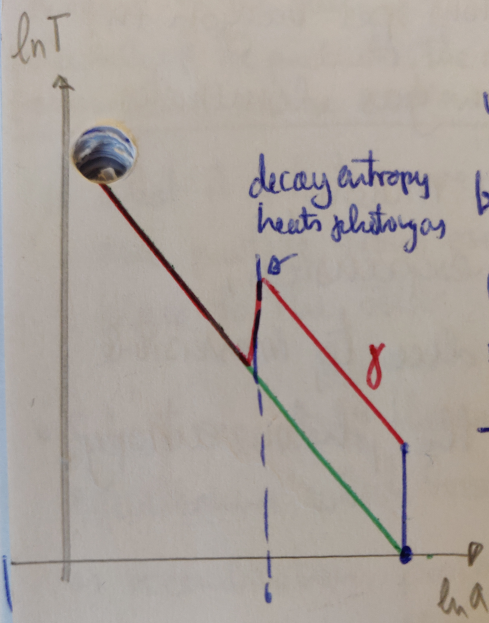
\includegraphics[width=0.5\linewidth]{gfx/neutrinoPhotonTemperature}
	\caption{}
	\label{fig:neutrinophotontemperature}
\end{figure}

\begin{mybox}{Temperature of photon and neutrino gas}
The temperature of the photon gas is therefore higher than that of the neutrino gas
\begin{equation}
\label{eq:photonAndneutrinoTemperature}
	T_\gamma = \left(\frac{11}{4}\right)^{\frac{1}{3}} T_\nu \approx 1.4 T_\nu,\quad \begin{array}{ll}
	T_\gamma = 2.726 K & \text{photons}\\
	T_\nu =1.95 K & \text{neutrinos} \\
	\end{array}.
\end{equation}
Hence the photon temperature is approx. $40\%$ higher today than the neutrino temperature.
\end{mybox}
\vspace{1cm}
What is then the contribution of the CNB to the full radiation energy density today $\Omega_{r,0,tot}$ ? \\
We know
\begin{equation*}
u \propto T^4\qquad \Omega_{r,0,\gamma}\approx 4\times10^{-5}
\end{equation*}
where the latter fact is from measurements. Including the statistical weights from neutrinos, we therefore have to replace
\begin{equation*}
	u_\gamma \rightarrow u_\gamma + \underbrace{3}_{species} \overbrace{\frac{7}{8}}^{=\frac{g_F}{g_B}\; fermion} \underbrace{\left(\frac{4}{11}\right)^{\frac{4}{3}}}_{\ref{eq:photonAndneutrinoTemperature}}u_\gamma = u_\gamma \left[1+\frac{21}{8} \left(\frac{4}{11}\right)^{\frac{4}{3}}\right].
\end{equation*}
Therefore, the neutrino contribution is given by
\begin{equation}
\Omega_{r,0,tot} = \Omega_{r,0,\gamma}\left[1+\frac{21}{8} \left(\frac{4}{11}\right)^{\frac{4}{3}}\right].
\end{equation}

\subsubsection{Photons and Baryons}
Baryons are non-rel. and therefore due to the Boltzmann suppression $n_B \propto e^{-T}$, much fewer in number than the relativistic species.\\
The number density of baryons $n_B$ and of photons $n_\gamma$ both scale with temperature $n_B,n_\gamma \propto T^3\propto a^{-3}$\footnote{Note that temperature of the universe means temperature of the photon gas and vice versa.}, hence their ratio $\eta$ \textbf{is constant}
\begin{equation}
	\eta = \frac{n_B}{n_\gamma} = 2.7 \times 10^{-8} \Omega_B h^2
\end{equation}
with
\begin{equation}
	n_B \propto \frac{\rho_B}{m_p}= \frac{\Omega_B}{m_p} \frac{3 H^2_0}{8 \pi \mG} = 1.1 \times 10^{-5} \underbrace{\Omega_B h^2}_{\approx 0.025} \;cm^{-3}
\end{equation}\footnote{assuming baryons are locked up in hydrogen}
and today
\begin{equation}
	n_\gamma=n_\gamma(T_{CMB}) =407 \; cm^{-3}.
\end{equation}
Thus, there are approximately a billion photons per baryon in the universe. The entropy of the photon gas dominates the entropy of the universe by a huge margin, justifying the assumption of adiabatic expansion, because any contribution to the entropy due to irreversible processes can be neglected compared to the photon entropy.




\subsubsection{The Recombination process}
The early universe was opaque to electromagnetic radiation, because of (Thomson) scattering by free electrons, as the mean free path each photon could travel before encountering an electron was very short. As the temperature drops, electrons and protons combine to form hydrogen atoms when the reaction
\begin{equation}
e^- + p^+ \leftrightharpoons H + \gamma 
\end{equation}
freezes out. This happens, because at lower temperature there are less high energetic photons to scatter the free electrons or to destroy the new hydrogen atoms. Then the photons decouple from matter, as their mean free path grew rapidly and became longer than the horizon distance. Then $e^-$ and $p^+$ recombine to hydrogen and the photons travel freely through the universe from there on known as \emph{cosmic microwave background} (CMB).\\
Before recombination, the strongest coupling between the photons and the rest of the plasma is through Thomson scattering
\begin{equation}
e^- + \gamma \rightarrow e^- + \gamma.
\end{equation}
The sharp drop in the free electron density after recombination means that this process becomes inefficient and the photons decouple.\\
\\
At what temperature did the freeze-out happen ?\\
We make the following approximations for this analysis:
\begin{enumerate}
	\item Overall number of particles stays fixed, i.e. canonical ensemble.
	\item All species are classical ideal gases composed of indistinguishable particles with densities low enough for degeneracy effects to be negligible.
	\item The photons do not contribute because they provide the heat bath controlling the temperature $T$.
	\item The inter-particle separation $\gg \lambda_B$ of particles involved, thus it is valid to compute the classical partition sum in phase space.
	\item The chemical potential must vanish in chemical equilibrium (compare \ref{eq:chemicalpotential})
	\begin{equation}
		\mu_e + \mu_p =  \mu_H,
	\end{equation}
	thus we have the Massenwirkungs-law in thermal equilibrium
	\begin{equation}
		\frac{Z_e Z_p}{Z_H} = \frac{N^2_e}{N_B - N_e}.s
	\end{equation}
\end{enumerate}
\begin{mybox}{Saha equation}
	We arrive at Saha's equation\begin{equation}
		\frac{x^2}{1-x} = \frac{(2 \pi m_e k_B T)^{\frac{3}{2}}}{(2\pi \hbar)^3 n_B} e^{-\frac{\chi}{k_B T}}
	\end{equation}
	with ionisation potential of hydrogen 
	\begin{equation}
		\chi = (m_e+m_p-m_H) c^2 = 13.6 eV
	\end{equation}
	and $x=\frac{N_e}{N_B}$ the \emph{ionisation degree} or \emph{free electron fraction}. 
\end{mybox}
\begin{figure}[h!]
	\centering
	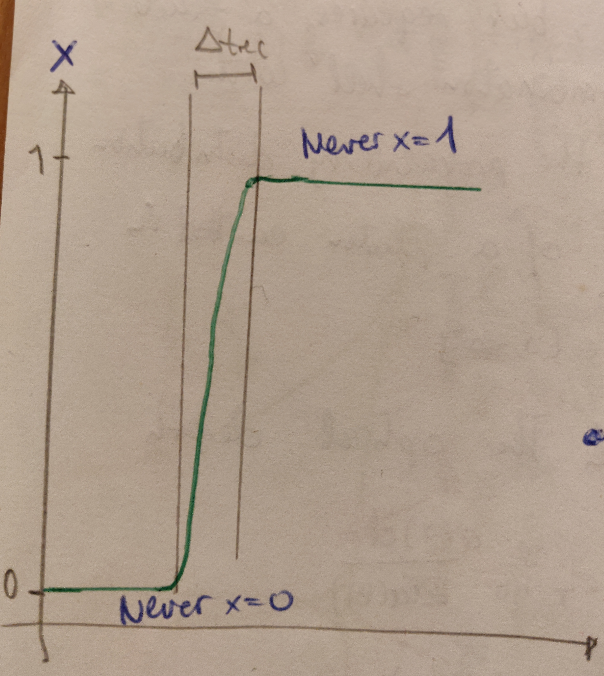
\includegraphics[width=0.5\linewidth]{gfx/sahaeq}
	\caption{}
	\label{fig:sahaeq}
\end{figure}



\begin{mybox}{Recombination epoch}
	This equation tells us that photons decoupled from matter at approximately
	\begin{equation}
	T_{rec} \approx 3400K.
	\end{equation}
	Since $\chi=13.6 eV$, one would naively expect $T_{rec} \approx10^5 K$. The very large photon-to-baryon ration $\eta^{-1}$ delays recombination considerably\footnote{Due to the Wien tail in the planck distribution of photons.}\\
	Once recombination starts, it happens very fast in a time period of approximately
	\begin{equation}
		\Delta t_{rec} \approx 40000 yr \quad \Leftrightarrow \quad \Delta z = 200.
	\end{equation}
	With $T_0 \approx 2.7K$ and $T_{rec}$ we find the scale factor at which recombination happened by noting that for ultra-rel. particles
	\begin{equation}
		T\propto a^{-1} \; \Rightarrow \; T =\frac{T_0}{a},\;\Leftrightarrow T_{rec} = \frac{T_0}{a_{rec}},
	\end{equation}
	which gives us (as $a_0=1$)
	\begin{equation}
		a_{rec} = \frac{T_0}{T_{rec}} \approx \frac{1}{1200}, \; z_{rec} \approx 1320, \; t_{rec} \approx 380000yrs
	\end{equation}
	after the Big Bang. With matter-radiation equality at $z_{eq} \approx 3500$, we conclude that \textbf{recombination occurred in the matter-dominated era}.
\end{mybox}\footnote{One has to include the $60\%$ neutrino contribution in CMB for correct results.}
Note the following comments on the recombination epoch:
\begin{enumerate} 
\item Note that Saha's equation assumes thermal equilibrium which breaks down as recombination proceeds. Still, it provides a very good approximation as $\Delta t_{rec}$ os very brief.
\item 
Why do we only see approx. one temperature of the decoupled photons, i.e. of the CMB ?\\
The photons released earlier at higher temperature are redshifted for a longer duration $\Rightarrow$ This evens the decoupled photons out in temperature such that all photons released at recombination arrive at the same energy, the same temperature today.
\item 
The Recombination process is also delayed by the following process:\\
Freshly formed hydrogen atoms can be ionized again by the recombination energy, by photons emitted from just then forming hydrogen atoms. The recombination energy is at least a Lyman-$\alpha$-photon and thus very energetic. Recombination can only proceed from this point onwards due to forbidden two-photon processes (e.g. $2s\rightarrow1s$).
\end{enumerate}
On the finite time-width of the Recombination epoch:\\
Recombination is not instantaneous, but requires a finite time interval. There is thus a \emph{recombination shell} with finite thickness. This can be analysed as follows. Imagine a photon escaping the cosmic plasma after being scattered off of an electron for the last time at a redshift depth $z$ inside the recombination shell (i.e. $Z$ corresponds to some geometrical depth $L$). One can quantify the probability distribution for last scattering at redshift $z$ of a photon emitted in the recombination shell
\begin{figure}[h!]
	\centering
	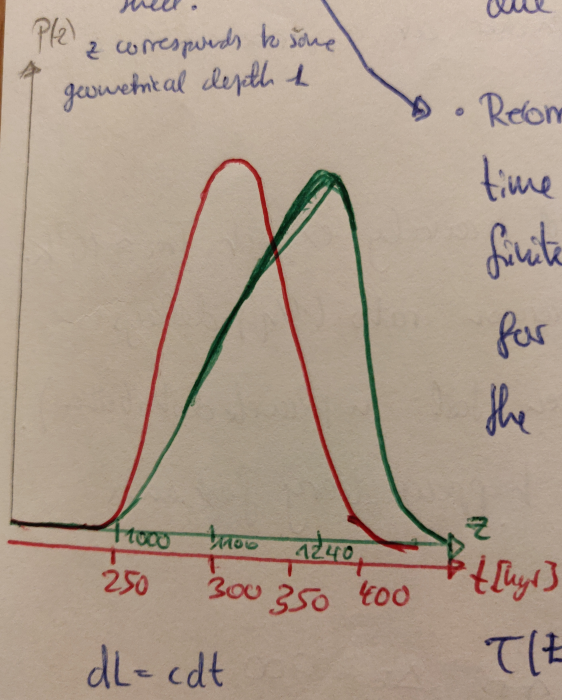
\includegraphics[width=0.5\linewidth]{gfx/RecombinationShell1}
	\caption{}
	\label{fig:recombinationshell1}
\end{figure}


\begin{equation}
	\frac{\md P(z)}{\md z} = \frac{\md \tau(z)}{\md z} e^{-\tau(z)},\qquad \tau \in[0,\infty] 
\end{equation}
with the \emph{optical depth} along a light ray in the recombination shell
\begin{equation}
	\tau(z) = n_e \sigma \int \md r = n_B \sigma T \int x \md r= - \int n_{B_0} (1+z)^3 [T_0 (1+z)] \sigma_T \frac{c}{H_0} \frac{a(z) \md z}{E[a(z)]}.
\end{equation}\footnote{The Thickness of the recombination shell is $\sigma_Z \approx 130$.}
The recombination shell is respective area as the backward lightcone (compare \ref{fig:recombinationshell}).
This $ \tau(z)$ is the optical depth of the recombination shell in the way that you ask how far you can go back into the recombination shell and find an electron that scatters on a photon for the last time. The probability distributions is Gaussian and centred around $z=1200$.
\begin{figure}[h!]
	\centering
	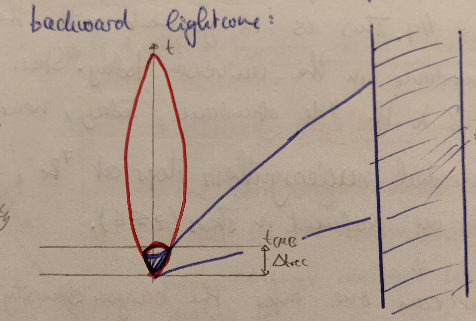
\includegraphics[width=0.5\linewidth]{gfx/recombinationShell}
	\caption{}
	\label{fig:recombinationshell}
\end{figure}
This shell is all the photons we see emitted in recombination. Thus, the probability for last scattering decreased exponentially after the recombination. The finite width of the recombination shell also shows, that the CMB photons were emitted at different $z$, as explained above they arrive all at the same redshift nevertheless.

\subsubsection{Nucleosynthesis}
Photons get hotter going back in time. This implies that there was a period of \emph{primordial nucleosynthesis} 
\footnote{Note for this analysis that the total number of nucleons stays constant due to baryon number conservation.}.\\
Photons and neutron are in thermal equilibrium until the reactions
\begin{equation}
	n+\nu_e \leftrightharpoons p+e^-,\quad n+e^+ \leftrightharpoons p+\bar{\nu}_e
\end{equation}
freeze out at $k_B T\approx 800 keV$. At this point, protons are way more common than neutrons, because neutrons are heavier. Until they're locked up again in $d, {}^4 He$ fusion processes at about $k_B T \approx 80 keV$, the neutrons decay furthermore, such that the neutron-to-proton ratio drops to
\begin{equation}
	\frac{n_n}{n_p}=\frac{1}{5} e^{-\frac{t}{\tau_n}} |_{t=5\text{ min}} = \frac{1}{7}
\end{equation}\footnote{Boltzmann distribution for decay of neutrons, takes $5$ mins. Protons and neutrons don't have the same number density in thermal equilibrium.}
\marginpar{$\tau_n=890 s$}
because neutrons decay for approximately $5$min until deuterium fusion sets in.
\begin{mybox}{Deuterium bottleneck}
	High photon density prevents ${}^2 H$ formation through photo dissociation until temperature has dropped well below $k_B T \approx 2$MeV corresponding to the binding energy. ${}^2 H$ formation is delayed until $k_B T\approx 80$keV at about three minutes after the Big Bang.
\end{mybox}
\begin{figure}[h!]
	\centering
	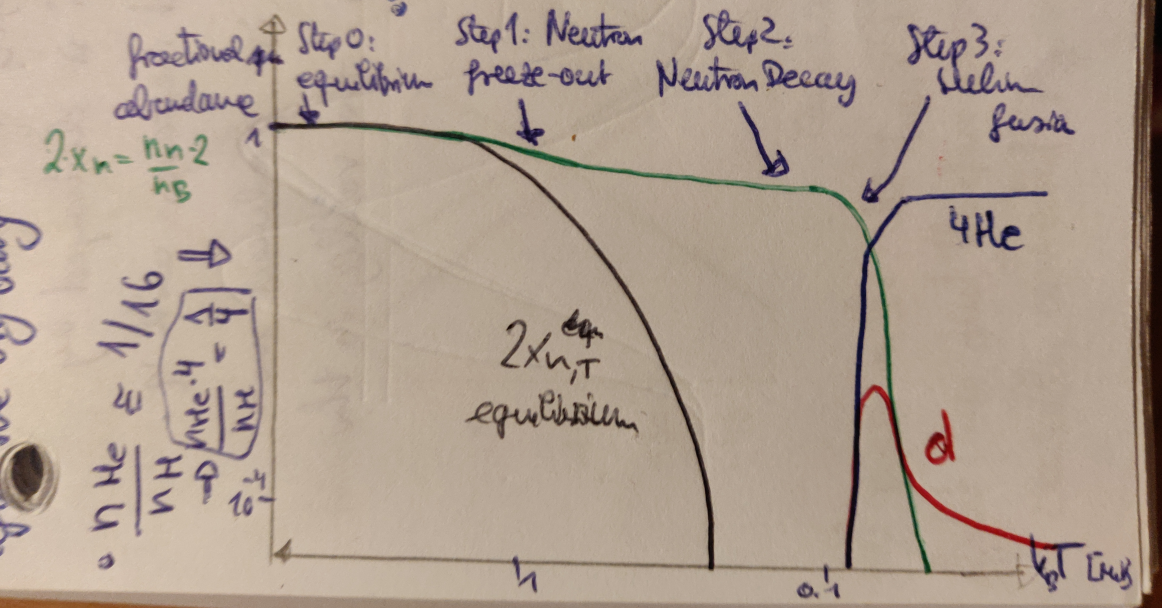
\includegraphics[width=0.5\linewidth]{gfx/nucleosynthesis}
	\caption{}
	\label{fig:nucleosynthesis}
\end{figure}
Big Bang nucleosynthesis began roughly $10$ seconds after the big bang, when the universe had cooled sufficiently to allow deuterium nuclei to survive disruption by high-energy photons (the neutron-proton freeze out time was earlier). At this point all free neutrons get locked up through a fusion chain into ${}^4 He$ because of its high binding energy. The expected ${}^4 He$ abundance by mass is $Y_P = \frac{1}{4}$ \footnote{$\frac{n_{He}}{n_H} \approx \frac{1}{16}$ implying $\frac{4 \cdot n_{He}}{n_H} = \frac{1}{4}$.}. This is in agreement with the measurement of ${}^4 He$ abundance in the universe today. Stars have only contributed $\approx 4\%$ to the ${}^4 He$ abundance today, nearly only primordial abundance.\\
Primordial nucleosynthesis stops at ${}^7 Be$, heavier elements are later on produced in stars ($z\leq 6$).
\begin{figure}[h!]
	\centering
	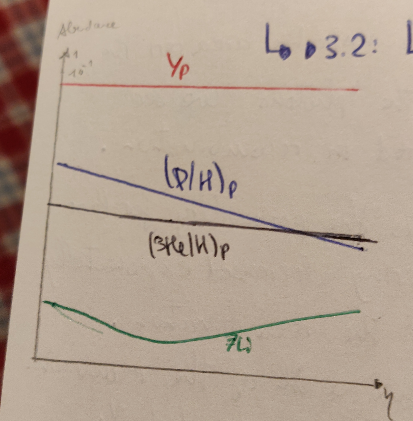
\includegraphics[width=0.5\linewidth]{gfx/nucleosynthesisAbundance}
	\caption{}
	\label{fig:nucleosynthesisabundance}
\end{figure}
\begin{mybox}{Lithium valley}
Description of \ref{fig:nucleosynthesisabundance}:\\
The abundance of ${}^4He$ increases with increasing $\eta$ as nucleosynthesis starts earlier for larger baryon density. $D$ and ${}^3 He$ are burnt by fusion, thus their abundances decrease as $\eta$ increases. Finally, ${}^7 Li$ is destroyed by protons at low $\eta$ with an efficiency that increases with $\eta$. On the other hand, its precursor ${}^7 Be$ is produced more efficiently as $\eta$ increases. This explains the \emph{Lithium valley} in the curve for ${}^7 Li$.
\end{mybox}
\vspace{1cm}
How can one infer the baryon density $\Omega_B$ of the universe from light element abundances ?\\
The abundances of light elements like helium, deuterium and lithium depend on the baryon-to-photon ratio $\eta$ which depends on the baryon density $\Omega_B$. Since deuterium has the strongest dependence on $\eta$, it gives the tightest constraints on $\Omega_B$.\\
Comparison with observations is difficult because light elements get produced and consumed (e.g. in stars) during cosmic history. Objects need to be found which either retain the primordial element mix, or in which abundance changes can be constrained.




























\newpage
\section{Cosmological Inflation}
\subsection{The horizon and flatness problem}
\subsubsection{Horizon problem}
The comoving radius of a sphere around a given point in the recombination shell which could have had causal contact with this point before recombination is
\begin{equation}
	\Delta \omega(0,t_{rec}) \approx 200 Mpc.
\end{equation}
The angular diameter-distance from us to the recombination shell is 
\begin{equation}
	D_{ang}(0,z_{rec}) \approx 6 Mpc.
\end{equation}
Thus, the angular size of the particle horizon \emph{at recombination} on the CMB sky is therefore
\begin{equation}
	\theta_{rec} = \frac{a_{rec} \Delta \omega(0,a_{rec})}{D_{ang}(0,a_{rec})} \approx 1.7^°.
\end{equation}
Given any point on the microwave sky, the causally connected region around it has a radius of approximately one degree.
\emph{How is it possible that the CMB is nearly isotropic ? Points on the sky further apart than $\approx 2^°$ had no chance of causally interacting and ’communicating’ their temperature}. This constitutes the \emph{Horizon problem}.\\
\\
From another POV, we can consider the Horizon problem via an analysis of our past lightcone, compare \ref{fig:horizonproblem}.
\begin{figure}[h!]
	\centering
	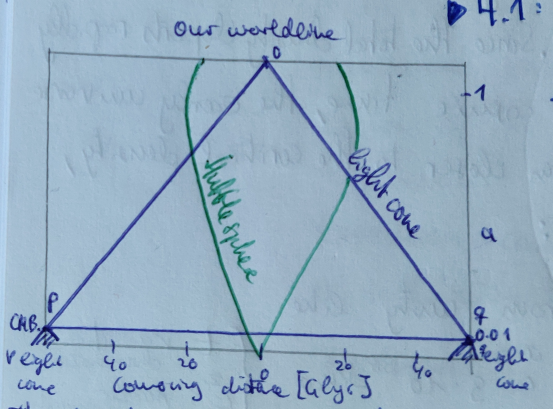
\includegraphics[width=0.7\linewidth]{gfx/horizonproblem}
	\caption{}
	\label{fig:horizonproblem}
\end{figure}
 The intersection of our past ligt cone with the spacelike slice labelled CMB corresponds to two opposite points in the observed CMB. their past light cones do not overlap before they hit the singularity $a=0$, so the points never have been in causal contact. The same applies to any two points in the CMB that are separated by more than $1$ degree on the sky.
\\
\\
This problem, as well as the Flatness problem as we will see below, can be solved by a period of inflation. Note that cosmological inflation is a model, it is proposed to solve these and other conundrums, but we have yet to measure the slow-roll parameters successfully, nothing is set in stone as of yet.\\
Inflation implies a phase of shrinking Hubble radius\footnote{The Hubble radius $r_H =\frac{c}{aH}$ is the comoving distance over which particles can travel in the course of one expansion time (the expansion time is the Hubble time $t_H = H^{-1} = \frac{\md t}{\md \ln a}\propto$ the time in which $a$ doubles).}. 
The past light cones of widely separated points in the CMB now (i.e. after a period of cosmological inflation) had enough time to intersect before $t=0$.



\begin{figure}[h!]
	\centering
	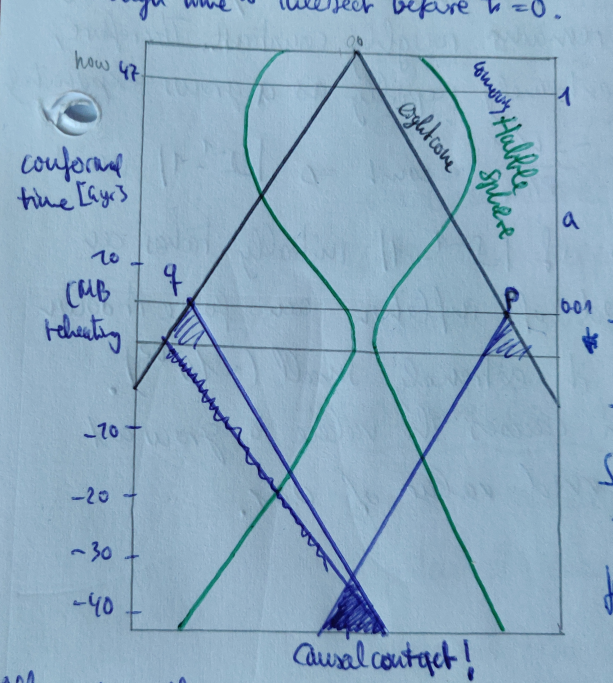
\includegraphics[width=0.7\linewidth]{gfx/Inflation}
	\caption{}
	\label{fig:inflation}
\end{figure}
All points in the CMB now have overlapping past light cones and therefore originated from a causally connected region of space.\\
\begin{mybox}{Idea of inflation}
	Summarizing, inflation is a mechanism to achieve 
	\begin{equation}
		\omega_{ph} \gg \frac{c}{a H} = r_H
	\end{equation}
	such that particles can not communicate now (or when CMB was created), but were in causal contact early on.
\end{mybox}


\subsubsection{Flatness problem}
This problem constitutes the fact that the spatial curvature of the universe is fine-tuned to a very special value and that small deviations from this value would have an extreme effect on the appearance of the universe.  The current density of the universe is observed to be very close to the critical value $\rho_{cr}$ required for flat universe. Since the total density departs rapidly from the critical value after cosmic time, the early universe must have had a density even closer to the critical density, departing from it by $\propto 10^{-62}$:
\\
The total density deviates from unity like
\begin{equation}
	\abs{1-\Omega_{tot}} = \frac{K c^2}{a^2 H^2(a)} \stackrel{a=a_{eq}}{\approx} 3\cdot 10^{-58} \Omega_{K,0} \; \left\{\begin{array}{ll}
	t & \text{radiation domination} \\
	t^{\frac{2}{3}} & \text{matter domination} \\
	\end{array}		\right\}.
\end{equation}
If there is any tiny deviation of $\Omega_{total}$ from unity at early times, it moves rapidly away from unity. In order for $\Omega_{total}$ to be anywhere near unity today, it must have been extremely close to unity at early times, which constitutes a \emph{fine-tuning problem}.
\\
Inflation provides a possible solution:\\
The proposed cause of inflation is a field which permeates spacetime and drives the expansion. the field contains a certain energy density, but unlike the density of matter or radiation present in the late universe, which decreases over time, the density of the inflationary field remains roughly constant. Therefore, the term $\rho a^2$ increases extremely rapidly as $a$ grows exponentially with
\begin{equation}
\left( \frac{1}{\Omega}-1  \right)\rho a^2 = -\frac{3 K c^2}{8 \pi \mG} = const. 
\end{equation}
$\Rightarrow \; \abs{\Omega^{-1}-1}$ must decrease with time. Thus, if $\abs{\Omega^{-1}-1}$ initially takes an arbitrary value, a period of inflation can force it down towards $0$ and leave it extremely small ($\approx 10^{-62}$). Subsequent evolution then causes the value to grow and bring it to the today observed value of $0.01$.

\subsection{The idea of inflation}
Accelerated expansions seems incompatible with gravity because the gravitational force exerted by the matter inside a representative spherical section of the universe is expected to decelerate its expansion.\\
Expansion can accelerate, i.e. $\ddot{a}>0$, if and only if the pressure is sufficiently negative
\begin{equation}
\stackrel{\ref{eq:friedmanneq2}}{\Rightarrow} \quad p< - \frac{\rho c^2}{3}.
\end{equation}
This is equivalent to shrinking the comoving Hubble radius
\begin{equation}
	\frac{\md}{\md t} \left(\frac{c}{a H}\right) <0.
\end{equation}
Thus, the idea of inflation also solves the flatness problem, because it could be solved if the comoving Hubble radius could shrink sufficiently for some time \footnote{The statement that our universe is expanding is equivalent to the statement that our field of view is getting narrower.}, because then the deviation of $\Omega_{total}$ from unity would be driven towards zero.\\ The Hubble radius characterizes the radius of the observable universe, thus the comoving Hubble radius gives the radius of the observable universe in comoving coordinates. If the comoving Hubble radius could shrink during some time, the observable part of the universe could be moved within causally connected regions, thus the contents of the entire observable universe could be brought into causal contact. After this phase ends, the observable universe can expand again, but its physical state can appear coherent everywhere thereafter, thus posing a solution to the horizon problem.
\subsubsection{Slow-Roll conditions for inflation to happen}
In this model, inflation ocurred by a scalar field rolling down a potential energy hill. When the field rolls very slowly compared to the expansion of the universe, inflation occurs. However, when the hill becomes steeper, inflation ends and reheating can occur.\\
Assume the inflaton field to be a scalar field with a finlaton potential $V(\phi)$, which has to be nearly constant
\begin{align}
	\mL &= - \half g^{\alpha \beta} \partial_\alpha \phi \partial_\beta \phi - V(\phi) \\
	\Rightarrow \quad T\munu&=\partial_\mu \phi \partial_\nu \phi+g\munu \left[-\half g^{\alpha \beta} \partial_\alpha \phi \partial_\beta \phi - V(\phi)\right]
\end{align}
with the total inflaton energy density
\begin{equation}
	\rho_\phi = \half \dot{\phi}^2 + V(\phi).
\end{equation}
The requirement for accelerated expansion resulted in the need for \textbf{negative pressure} 
\begin{equation}
\ddot{a} >0 \quad \Rightarrow \quad p < -\frac{\rho c^2}{3}.
\end{equation}
How do you get this ? For the inflaton field introduced, this can be achieved, if it satisfied the following conditions
\begin{align}
	\frac{\dot{\phi}^2}{\hbar c^3} & \ll V \text{ $\phi$ has to move sufficiently slow}\label{eq:slowroll1}\\
	\ddot{\phi} & \ll \frac{\md V(\phi)}{\md \phi}.\label{eq:slowroll2}
\end{align}
These imply for the equation of state $P = w \rho  c^2$:
\begin{equation}
	w= \frac{\frac{\dot{\phi}^2}{2 \hbar c^3} -  V}{\frac{\dot{\phi}^2}{2 \hbar c^3} + V}
\end{equation}
which has the lower bound $w\rightarrow -1 $ for a still standing field $\frac{\md \phi}{\md t}=0$. Thus, with the condition \ref{eq:slowroll1} $w$ gets sufficiently negative and we arrive at negative pressure, thus repulsive gravity.\\
\\
A successful inflationary phase (the conditions stated above) can be phrased in terms of the conditions for the slow-roll parameters.
\marginpar{$E_{pl} = m_{pl} c^2 = \sqrt{\frac{\hbar c^5}{\mG}}$, $V^\prime := \frac{\md V(\phi)}{\md \phi}$}
\begin{mybox}{Slow-roll conditions}
\begin{enumerate}
	\item Inflation occurs only if the kinetic energy $\frac{\dot{\phi}^2}{2}$ only makes a small contribution to the total energy $\rho_\phi$:
	\begin{equation}
\epsilon := \frac{E^2_{pl}}{16 \pi \mG} \left( \frac{V^\prime}{V}\right)^2 \ll 1.
	\end{equation}
	This condition says, that the slope of the potential has to be small in comparison to the potential. This reads as $V\approx$constant during inflation, i.e. during inflation the Hubble function is essentially constant
	\begin{equation}
		H\approx \text{constant} !
	\end{equation}
	The $\epsilon$ condition is needed for an inflation epoch to start in the first place.
	\item 
	\begin{equation}
		\eta := \frac{E^2_{pl}}{8 \pi \mG} \left(\frac{V^{\prime \prime} }{V}\right) \ll 1.
	\end{equation}
	This condition says that $V$ is essentially flat w.r.t. $\phi$. Thus it says that the first conditions has to hold for a long time. This conditions is needed for an inflation epoch to last.
\end{enumerate}
\end{mybox}
The condition that the two slow-roll parameters $\epsilon$ and $\eta$ be much smaller than unity indicates that both the slope and the curvature of the inflaton potential have to be small in order to generate a substantial negative pressure that results in a period of accelerated expansions that is strong enough and that lasts long enough in order to solve both the horizon and flatness problem.\footnote{It is way more difficult to construct a potential that satisfies the $\eta$ condition than the $\epsilon$ condition, this is known as the \emph{eta-problem}.}\\
\\
Thus with $H(a)\approx$constant during inflation, the comoving Hubble radius $\frac{c}{aH}$ has to shrink during this epoch, because $a$ increases with time. This was the required criterion to solve the flatness problem. By an estimate in order for inflation to solve the flatness problem, the comoving Hubble radius had to shrink by $\approx 10^30$, which corresponds to an increase in the scale factor by approximately $e^{60}$. This solves the causality problem at the same time, because before inflation one has a tiny patch of observable domains in thermal equilibrium which is then inflated exponentially. Then one ends up with an observable universe which appears to be in thermal equilibrium.\\
\\
Since th densities of observable quantities scale like $\rho_r \propto a^{-4}$, $\rho_m \propto a^{-3}$, all other densities than the energy density of the inflaton field (which is approximately constant during inflation, since $\rho c^2 \approx V$ and the changes in $V$ are small due to slow-roll conditions) drop by huge amounts.\\
 Since there is matter and radiation in the universe today, there must a way to convert the energy density of the inflaton field into the energy density of radiation or matter as inflation ends, i.e. when $(\epsilon,\eta)\approx 1$.\\
 It is assumed that the inflaton field can decay through some coupling to ordinary matter and thus turn its energy density back into other constituents of the cosmic fluid $\Rightarrow$ \emph{reheating process}. \textbf{This is an open question}.

\subsubsection{Inflation and structure formation}
Once inflation sets in, the vacuum fluctuations of the inflaton field due to the uncertainty principle are quickly driven outside of the horizon (i.e. the horizon quickly contracts below the length scale of the quantum fluctuations), where they "freeze in" because they lack causal contact.\\
\paragraph{Idea of Inflation originating cosmic structures}
Like any other quantum field, the inflaton field must have undergone microscopic vacuum fluctuations due to Heisenberg's uncertainty relation. As inflation started, the wavelengths of these fluctuations grew so large that they became larger than the horizon at that time\footnote{In terms of comoving distance, the particle horizon is equal to the conformal time $\eta$ that has passed since the Big Bang.}. As a result, thee now largely microscopic fluctuations lose their causal connection, cannot decay any more and therefore freeze in. These fluctuations then serve as a seed for the structures in the Universe that we can observe today.\\
\\
The model for density fluctuations produced in this way is described crudely in the following:
\begin{enumerate}
	\item Introduce a conformal time $\md \eta$ for the inflationary epoch, i.e. $\eta \in (-\infty,0)=$ (beginning inflation, end inflation). With $H\approx constant$ during inflation one finds
	\begin{equation*}
		\md s^2 = a^2(\eta) \left[-\md \eta^2 + \md \vec{\omega}^2\right] \quad \Rightarrow \quad a \md \eta = c \md t
	\end{equation*}
	such that
	\begin{equation*}
		\eta = - \frac{c}{H a} \quad [\md \eta] = \text{length} \Rightarrow \; \mathcal{H} (\eta):= \frac{a}{c} H.
	\end{equation*}
\item Make a mean field ansatz for the inflaton field by decomposing it into a smooth part $\varphi_c$ and a part $\varphi$ responsible for fluctuations
\begin{equation}
	\varphi \rightarrow \phi_c + \varphi.
\end{equation}
Fluctuations of the field imply fluctuations of the metric. By Einsteins equations one finds a modified Poisson equation
\begin{equation}
	\frac{\md^2 u}{\md \eta^2} - \frac{\left(\frac{\md^2 z}{\md \eta^2}\right)}{z} u - \vec{\nabla}^2 u = 0,\quad z= \frac{a^2}{a^\prime}\phi^\prime_c,\; u=a \varphi + \phi z.
\end{equation}
By imposing the slow-roll conditions and only perturbing to the $1^{st}$ order, one can approximate this field equation. One finds a free mode expansion of the field $u\approx a \varphi$, thus of the fluctuations, by this approximation ($V$ is assumed to be nearly constant). The solution through a Fourier transform reads
\begin{equation*}
	u^\pm_k = u^{(0)}_k e^{\pm i k \eta} \left(1 \pm \frac{i}{k \eta}\right) \; \Rightarrow \; \varphi^\pm_k = \varphi^{(0)}_k \frac{H}{ck} e^{\pm i k \eta} \left[i \pm k \eta\right].
\end{equation*}
These are the inflaton fluctuations, \emph{Bunch-Davies modes}.
\item With this result, one can make the case distinction
\begin{mybox}{}
	\begin{enumerate}
		\item $\abs{k \eta} \ll 1 \Rightarrow \varphi^\pm_k\approx constant$ (i.e. freeze-in) \emph{and} $\lambda \gg$ Horizon ($\frac{k c}{H} \ll 1$).
		\item $\abs{k \eta} \gg 1 \Rightarrow \varphi^\pm_k$ oscillating very fast \emph{and} $\lambda \ll$ Horizon ($\frac{k c}{H} \gg 1$).
	\end{enumerate}
\end{mybox}
\item Thus, by the exponential expansion of inflation, $k$ grows greatly beyond the horizon. In the horizon, the modes oscillate and they freeze-in after being driven out of the horizon. Thus in the horizon inflaton and anti-inflaton particles are causally connected, such that they recombine and fluctuations disappear. They are no longer causally connected outside of the horizon, such that they cannot recombine anymore and the fluctuations stay after being driven out of horizon. Then, out of horizon with $\lambda \gg$Horizon, the inflaton fluctuations are 
\begin{equation*}
	\tilde{\varphi}^\pm_k=\varphi^{(0)}_k \frac{H(t_X)}{c k},
\end{equation*}
where $t_X$ is the time of modes crossing the horizon.
\item In order to estimate the size of the remaining fluctuations outside of the horizon one has to evaluate the amplitude of the field. This can be done via the vacuum expectation value of the inflaton field
\begin{equation}
\expval{\tilde{\varphi}^\pm_k}{0} = \varphi^{(0)}_k= \frac{E^{\frac{3}{2}}_{pl}}{\sqrt{2 \hbar c k} }.
\end{equation}
Then the amplitude of which inflaton modes on average freeze out as they leave the horizon is then
 \begin{equation}
 	\expval{\abs{\tilde{\varphi}^\pm_k}^2}{0} = \frac{E^3_{pl}}{2 \hbar c^3} \frac{H(t_X)}{k^3}, \quad H(t_X)\approx H_k.
 \end{equation}
 \item In the next step one wants to find the \emph{(primordial) density power spectrum}. Therefore one wants to derive a relation between the density fluctuations, Fourier modes and the fluctuations today. Thus something like 
 \begin{equation*}
 	(\text{inflaton fluctuations}(k))\propto (\text{cosmic density fluctuations}(k)).
 \end{equation*}
One finds
\begin{equation}
	\delta := \frac{\delta \rho}{\rho} = \frac{2 \cdot 16 \pi}{E^2_{pl}} \frac{V}{\frac{\md V}{\md \varphi_c}} \cdot \varphi. 
\end{equation}
Therefore the amplitude of mean density fluctuations is 
\begin{equation}
	\expval{\abs{\left(\frac{\delta \rho}{\rho}\right)_k}^2}{0} = \frac{4}{3} \frac{1}{E_{pl}} \frac{V}{k^3 \epsilon} |_{k=a H},
\end{equation}
which is evaluated at the time where modes with $k$ crossed the horizon and freezes in.\\
Therefore we find that the density fluctuations depend on $k$, i.e. they have a defined spectrum. This is the \emph{density power spectrum} $P(k)$, which says how much of the signal (e.g. of CMB) is at wavenumber $k$
\begin{equation}
	P(k)=\abs{\hat{\delta}(\vec{k}) }^2.
\end{equation}
\paragraph{Comment on matter power spectrum, may remove later if added in structure formation}
The matter power spectrum describes the density contrast of the universe (the difference between local and mean density) as a function of scale. It is the Fourier transform of the matter correlation function. On large scales, gravity competes with cosmic expansion and structures grow according to linear theory. In this regime, the density contrast field is Gaussian, Fourier modes evolve independently, and the power spectrum is sufficient to completely describe the density field. On small scales, gravitational collapse is non-linear, and can only be computed accurately using $N$-body simulations.
\item The scalar power spectrum is formally defined as
\begin{equation}
\mathcal{P}_S := \frac{k^3}{2 \pi^2} \expval{\left(\frac{\delta \rho}{\rho}\right)^2_k}.
\end{equation}
\item The modes caused by the inflationary expansion of quantum fluctuations are called \emph{scalar modes}. Their power spectrum is with the above result
\begin{equation}
	\mathcal{P}_S = \frac{2}{3\pi^2 E_{pl}} \left(\frac{V}{\epsilon}\right)_{k=aH},
\end{equation}
again evaluated at the point when modes left horizon.
\item This scalar power spectrum has an exponent close to one
\begin{equation}
	\frac{\md \ln \mathcal{P}_S}{\md \ln k} = - 6 \epsilon +2 \eta \equiv n_s -1 \quad \Rightarrow\quad P_S = A k^{n_s}, \; A=const.
\end{equation}
The index of $\mathcal{P}_S,n_s$, can now be measured, thus a linear combination of the slow-roll parameters can be measured, this is one possibility to test inflation.
\item Fluctuations in the inflation field result in fluctuations in the metric. This results in gravitational waves, the so-called tensor-modes. Thus, the tensor modes also have a power spectrum
\begin{align}
	\mathcal{P}_t &= \frac{3^2}{\epsilon \pi^2 E_{pl}} V|_{k=aH} = \tilde{A}k^{n_t} = \tilde{A} k^{-2 \epsilon} \nonumber \\
	\Rightarrow \quad \frac{\md \ln \mathcal{P}_t}{\md \ln k} &= -2 \epsilon \equiv n_t \nonumber \\
	\Rightarrow \quad \frac{\mathcal{P_t}}{\mathcal{P}_s} &=16 \epsilon =: r.
\end{align}
\item Thus there are three quantities measurable to prove inflation
\begin{align}
	n_s &= 2 \eta - 6 \epsilon +1 \\
	n_t &= -2 \epsilon\\
	r&= 16 \epsilon.
\end{align}
\begin{mybox}{How to validate Inflation}
	Inflation makes the following observable predictions
	\begin{enumerate}
		\item The initial scalar perturbations should have a nearly Gaussian nature. This was confirmed with the temperature fluctuations in CMB.
		\item The scalar perturbations should have a spectral index, that is almost unity. Its deviation from unity is given by a combination of the slow-roll parameters. This small deviation from unity was actually observed.
		\item Primordial gravitational waves with an almost flat spectrum are predicted; their spectral index should be given by $-2 \epsilon = n_t$.
		\item The ration between tensor and scalar perturbations should be given by $16\epsilon =r$.
	\end{enumerate}
	Until now, primordial gravitational waves have not yet been observed without a doubt.
\end{mybox}

\end{enumerate}


















\subsection{Dark Energy}
What is the mechanism that drives accelerated expansion of the Universe today ?\\
Two possible forms
\begin{enumerate}
	\item One form of dark energy could be the cosmological constant, representing a constant energy density filling space homogeneously.
	\item A quantum scalar field, dynamic quantities whose energy density can vary in time and space. One possibility is the \emph{quintessence field}.
\end{enumerate}
Comments on the above possibilities are in order.
\subsubsection{On inflation as dark energy}
It is not possible to regard the inflaton as the driving mechanism of accelerated expansion today, because it decayed at the end of inflation.
\subsubsection{On the role of dark energy as byproduct of the universe or of dark energy}
The occurence of $\Lambda$ and $\mG$ in a $4$-dimensional metric theory of gravity is perfectly natural as explained by Lovelock's theorem.
\subsubsection{Self-interacting scalar field}
A self-interacting scalar field would produce the negative pressure necessary for accelerated expansion
\begin{equation}
w= \frac{\frac{\dot{\phi}^2}{2 \hbar c^3} -  V}{\frac{\dot{\phi}^2}{2 \hbar c^3} + V}.
\end{equation}
One suggestion for the interaction potential of quintessence is the \emph{Ratra-Peebles potential}
\begin{equation}
	V(\phi) = \kappa \left(\frac{\phi_0}{\phi}\right)^\alpha.
\end{equation}
We find that for $\alpha > -2$ this quintessence field dominates at late times and leads to accelerated expansion. This RP. potential is favourable because of its \emph{tracker properties}: A wide variety of initial conditions for $\phi,\dot{\phi}$ lead to the same final solution for $\phi$.\\
\\
In all these possible models one has to consider time dependent equation of state parameters as well, such as
\begin{equation}
	w=w_0 +(1-a) w_a,
\end{equation}
which is called \emph{CPL-parametrization}. One observes \begin{equation}
	(w_0,w_a) \approx (-1,0)
\end{equation}
today (which is cosmological constant), a clear deviation would imply that accelerated expansion is \emph{not} driven by the cosmological constant.


\section{Evolution of cosmic structures}

\subsection{Linear perturbation theory}
Here we describe the basic theory for structure growth in the expanding universe. With the inhomogeneities being much smaller than the typical scale of the universe, we can neglect effects of GR/curvature and finite speed of information propagation and work with Newtonian dynamics and classical Hydrodynamics (fluid approximation).\\
We thus describe inhomogeneities in a cosmic fluid\footnote{Ideal fluids here, i.e. set of mass points with infinitely small mean free path (obvs. not true for cosmic fluids, but ok approximation in large scale regime).} which contains at least radiation, dark and baryonic matter and which moves according to Newtonian gravity:\footnote{Consider thus a non-relativistic fluid with mass density $\rho$, pressure $P\ll \rho$ and velocity $\vec{v}$.}
\begin{mybox}{Euler-Poisson equations}
	Energy-momentum conservation of a cosmic fluid $\partial_\mu T^{\mu \nu}=0$ is stated by the Euler-Poisson equations
	\begin{align}
		\frac{\partial \rho}{\partial t} + \vec{\nabla} \cdot (\rho \vec{v}) &= 0 \quad \text{mass conservation} \\
		\frac{\partial \vec{v}}{\partial t} + (\vec{v}\cdot \vec{\nabla}) \vec{v} &= - \frac{\vec{\nabla} P}{\rho} - \vec{\nabla}\Phi \text{  momentum conservation}\\
		\vec{\nabla}^2 \Phi &= 4 \pi \mG \rho.
	\end{align}
\end{mybox}
We want to find such a set of equations solely for the fluctuations parts of the $\rho,\vec{v}$ fields. We hence decompose the velocity and density field into their homogeneous background values, indicated by subscript $0$, and small perturbations

\begin{equation}
	\rho = \rho_0 (1+\delta), \; \vec{v}=\vec{v}_0+a \vec{u}, \; \Phi=\Phi_0+\phi.
\end{equation}
These are given in \emph{comoving coordinates} $\vec{r}=a(t) \vec{x}$, i.e.
\begin{equation*}
	\frac{\md}{\md t}(a \vec{x}) = \underbrace{\dot{a} \vec{x}}_{\text{Hubble flow}} + \underbrace{a \dot{\vec{x}}}_{\text{peculiar velocity}}
\end{equation*}
with the \emph{relative density contrast}
\begin{equation}
	\label{eq:densitycontrast}
	\delta = \frac{\delta \rho}{\rho}.
\end{equation}
\begin{mybox}{Linear perturbation equations}
	By only considering perturbations up to first order we find three perturbation equations
	\begin{align}
		(C) \quad \dot{\delta}+\vec{\nabla}\cdot \vec{u} &=0\\
		(E) \quad \dot{\vec{u}} + 2 H \vec{u} &= - \frac{\vec{\nabla}P}{a^2 \rho_0} - \frac{\vec{\nabla}\phi}{a^2} \\
		(P) \quad \vec{\nabla}^2 \phi &= 4 \pi \mG \rho_0 \delta a^2\\
		&\Leftrightarrow \frac{\delta \hat{\phi}}{c^2}=-\frac{3}{2} \frac{k^2_0\hat{\delta}}{k^2 a} |_{k^2_0\equiv\Omega_{K,0}H^2_0/c^2},
	\end{align}
where $(C)$ implies that particles must stream together to form density correlations.
\end{mybox}
We find an equation of state linking the pressure fluctuations to the density fluctuations
\begin{equation}
	 P=c^2_s \rho_0 \delta,
\end{equation}
\footnote{Not exactly correct, because $c_s$ has to be taken under adiabatic conditions, an adiabatic index is missing here.}
where $c_s=0$ for linearized CDM fluctuations.

\subsubsection{Density perturbations}
By combination of the perturbation equations one finds
\begin{align}
\ddot{\delta}+ 2 H \dot{\delta} &= \left[4 \pi \mG \rho_0 + \frac{c^2_s}{a^2} \vec{\nabla}^2\right]\delta,\\
\ddot{\delta}_k + 2 H \dot{\delta}_k &= \left[4 \pi \mG \rho_0 - \frac{c^2_s k^2}{a^2}\right]\delta_k, \nonumber \\
 \text{using       } \delta(\vec{x},t) &= \int \frac{\md^3 k}{(2 \pi)^3} \delta_k(\vec{k},t) e^{-i \vec{k}\cdot \vec{x}}\nonumber.
\end{align}
\begin{enumerate}
	\item One finds a d'Alembert equation for sound waves by dropping $\dot{\delta}$ and gravity term.
	\item By dropping $\dot{\delta}$ and $\vec{\nabla}^2$ one finds an exponentially growing oscillator, this describes the growth of cosmic structure.
\end{enumerate}
$2H \dot{\delta}$ is a damping term guaranteeing that cosmic structure growth goes as a power law, not exponentially. In case $1)$ this damping term dissipates the sound waves.

Below Jean's length, the fluctuations oscillate with decreasing amplitude. Above the Jeans' length, the fluctuations experience power-law growth, rather than exponential growth due to the damping term.





























\subsection{Linear growth factor, perturbations within and outside the horizon}
\subsection{Velocity perturbations and Zel'dovich approximation}
\subsection{Nonlinear evolution and power spectra}
\subsection{The Cosmic Microwave Background}
\subsubsection{The Dipole}
\begin{mybox}{}
	The Earth is not at rest with respect to the CMB.
\end{mybox}
Its motion around the Sun, combined with the Sun's motion around the centre of the Milky way, and so on, causes an effective net motion with velocity $v$ with respect to the CMB.
\begin{mybox}{CMB Dipole}
	This motion causes a dipolar pattern in the CMB temperature,\begin{equation}
		T_{obs} = T_{CMB,0} \left[1+\frac{v}{c} \mu\right] + \mathcal{O}\left(\frac{v^2}{c^2}\right), \quad \mu = \cos\angle(\vec{n},\vec{v}).
	\end{equation}
	The amplitude of the Dipole is, with the Earth's velocity being $v_{Earth} \approx 371 \frac{km}{s}$,
	\begin{equation*}
		T(v_{Earth}) \approx 10^{-3}K.
	\end{equation*}
\end{mybox}
The cosine of the angle between the line-of-sight and the direction of motion. The CMB temperature is slightly enhanced towards the direction of motion, and decreased in its anti-direction, corresponding to the Doppler shift of CMB photons.\\
Thus, one has to remove the mean value/background noise of the galactic plane and everything else and the Dipole from the CMB measurement to find the bare CMB with fluctuations of
\begin{equation}
	\frac{\Delta T}{T} \approx 10^{-5}.
\end{equation}
The density contrast at decoupling was of the order $\delta(a_{CMB}) \approx 10^{-3}$, we would therefore expect the CMB fluctuations to be of order $10^{-3}K$. The observed order of $10^{-5}K$ can be explained through the existence of not electromagnetically interacting dark matter.
\subsubsection{Perturbation equations and the Sachs-Wolfe effect}
Regarding initially only the ultra-rel CMB photons, we have
\begin{align}
	n &\propto T^3, \quad u \propto T^4, \quad P=\frac{u}{3} \propto T^4 \\
	\Rightarrow \quad \frac{\delta n}{n_0}& = 3 \theta,\quad \frac{\delta u}{u_0} = \frac{\delta p}{p_0} = 4\theta.
\end{align}
with the \emph{relative temperature fluctuation} $\theta=\frac{\delta T}{T_0}$.\\
From this we find using the continuity and Euler equation
\begin{align}
\ddot{\theta} -\frac{c^2}{3} \vec{\nabla}^2 \theta - \frac{1}{3} \vec{\nabla}^2\delta \phi &=0 \\
\ddot{\theta}_K + \frac{c^2 k^2}{3} \theta_k + \frac{k^2}{3} \delta \phi_k &=0.
\end{align}


 \todo{To finish.}




\section{Gravitational Lensing}
\subsection{Gravitational Lensing Equation from GR}
\subsection{Thin gravitational lenses}
\subsection{Correlation functions (no thin lens approximation)}
\section{Theoretical Astrophysics}








\newpage
\section{Two examples of Relativistic Astrophysics}
\subsection{Gravitational Lensing - TO COMPLETE FROM SCRIPT}
Consider a congruence/bundle of geodesics and calculate the propagation of light in the vicinity of a mass in order to quantify the effects of gravitational lensing. Pick a fiducial light ray from the light bundle with a normal vector $n$ perpendicular to its four-velocity measuring the distance to the other light rays in the bundle, i.e. its amplitude measure the diameter of the cross section of the light bundle.\\

\begin{figure}
	\centering
	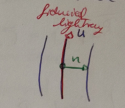
\includegraphics[width=0.7\linewidth]{gfx/gravlensingLightcongruence}
	\caption{}
	\label{fig:gravlensinglightcongruence}
\end{figure}
The Jacobi equation of geodesic equation reads:
\begin{equation}
\nabla^2_u n = \bar{R}(u,n)u.
\end{equation}
For a lightray introduce an affine parameter parametrizing the geodesic, since $\tau=0$ for light. Now, for a bundle of null-geodesics with the wavevector $\tilde{k}$ of the fiducial light ray:
\begin{equation}
\nabla^2_{\tilde{k}} n = \bar{R}(\tilde{k},n)\tilde{k},
\end{equation}
i.e. \emph{light bundles are deformed by the gravitational tidal field.}\\
\\
Note: Observer moving with $u_0$ seeing lightray measures frequency $\omega_0=\langle k, u_0 \rangle$, with $\tilde{k}:= \frac{k}{\omega_0}$.\\
\\
\subsubsection{Introduction of 2d Sachs space}
construct coordinate space $\perp \tilde{k}$ and also $\perp u_0 \Rightarrow$ 2d space in 3 space of observer, where it is perpendicular to lightray $\Rightarrow$ 2d screen perpendicular to light ray. $E_1,E_2$ span screen at the observer. Shift along lightray by parallel transport: $\nabla_{\tilde{k}}E_i=0$ and $\langle E^i,E_j \rangle = \delta^i_j; i,j \in \{1,2\}$, the \emph{Sachs basis}.\\
\begin{figure}
	\centering
	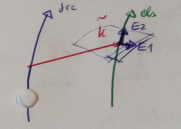
\includegraphics[width=0.7\linewidth]{gfx/gravlensingSachsbasis}
	\caption{}
	\label{fig:gravlensingsachsbasis}
\end{figure}

Also $\tilde{k} \propto k $ null: $\langle \tilde{k},\tilde{k} \rangle =0$ and null geodesics $\nabla_{\tilde{k}} \tilde{k} =0$. With $n = N^i E_i$ inserted into the geodesic deviation equation
\begin{equation}
\nabla^2_{\tilde{k}} N^i =\underbrace{ \langle E^i, \bar{R}(\tilde{k},E_j) \tilde{k} \rangle}_{=R_{\alpha \beta \gamma \delta} E^{i \alpha} \tilde{k}^{\beta} \tilde{k}^{\gamma} E^{\delta}_g} N^j .
\end{equation}
\begin{mybox}{Split up Riemann tensor }
	\begin{equation}
	\bar{R}_{\alpha \beta \gamma \delta} = \bar{C}_{\alpha \beta \gamma \delta} + g_{\alpha [\gamma} R_{\delta ] \beta} - g_{\beta [\gamma} R_{\delta] \alpha} - \frac{\mathcal{R}}{3} g_{\alpha [\gamma} g_{\delta] \beta}.
	\end{equation}
	The Weyl tensor $\bar{C}_{\dots}$ is equal to the Riemann tensor the vacuum solution of Einstein equations. It tells you which freedom you have in the Riemann tensor if you fix the Ricci tensor. The Weyl tensor is trace-free. The Weyl tensor corresponds to the gravitational tidal field and gives us the freedom left in geometry for fixed Ricci:
	\begin{equation}
	\bar{C}^{\alpha}_{\beta \alpha \delta} = 0, \quad \bar{C}_{\alpha \beta \gamma \delta} = - \bar{C}_{\beta \alpha \gamma \delta} = - \bar{C}_{\alpha \beta \delta \gamma}= \bar{C}_{\gamma\delta \alpha \beta}.
	\end{equation}
	One of the most important properties of the Weyl tensor is that it is invariant under conformal transformations. This means that if you compute $\bar{C}_{ρσμν}$ for some metric $g_{μν}$ , and then
	compute it again for a metric given by $Ω^2 (x) g_{μν}$ , where $Ω(x)$ is an arbitrary nonvanishing
	function of spacetime, you get the same answer. For this reason it is often known as the
	“conformal tensor.”
	The Weyl tensor vanishes in a homogeneous and isotropic universe, since it otherwise would induce a preferred direction. The Weyl tensor is responsible for distortions of the light bundle, which can not take place in an isotropic and homogeneous universe $\Rightarrow$ split up background and non-background action on light bundle.
	Note:
	\begin{equation}
	\phi_{ij} \rightarrow \phi_{ij} - \delta_{ij}\tr \phi_{ij} \frac{1}{3} = \underbrace{\phi_{ij}- \frac{4 \pi \rho}{3} \rho \delta_{ij}}_{\propto \bar{C}}
	\end{equation}
	which corresponds to a tidal field without matter (in Newtonian analogy). Note that the term $\propto \rho$ is the local matter. It describes the matter distribution around a light bundle as if beam were empty.
\end{mybox}
Inserting this form of the Riemann tensor into the geodesic deviation equation yields the optical tidal matrix $\mathcal{T}$:
\begin{equation}
\nabla^2_{\tilde{k}} N^i = \left[-\half R(\tilde{k},\tilde{k})\delta^i_j + \underbrace{C^i_j}_{\bar{C}_{\alpha \beta \gamma \delta} E^{i\alpha} \tilde{k}^{\beta} \tilde{k}^{\gamma} E^{\delta}_j} \right],
\end{equation}
where the former terms leads to an isotropic contraction or expansion of the light bundle cross section:
\begin{equation}
\nabla^2_{\tilde{k}} \vec{N} = \mathcal{T} \vec{N}.
\end{equation}
The Weyl tensor completely vanishes in an isotropic and homogeneous universe. Not perfect Friedmann universe $\Rightarrow$ We have fluctuations around the background which lead to Weyl fluctuations. Here , the Weyl tensor can be projected onto the tidal field of the Newtonian gravitational potential.\\
What happens for a light-bundle travelling through an unperturbed Friedmann universe ? $\Rightarrow \bar{C}=0$, i.e. ignore \emph{gravitational shear} (e.g. circular sections won't become elliptic. Ellipsis are not allowed in a Friedmann universe).
\subsubsection{Circular light bundle}
For circular light bundle (will remain circular since $C=0$). Check script for the case of $\bar{C}\neq 0$.
\begin{equation}
\nabla^2_{\tilde{k}} D = \kappa D.
\end{equation}
Expressing the Ricci tensor i.t.o. the Einstein tensor and field equation
\begin{equation}
R(\tilde{k},\tilde{k}) = G(\tilde{k}, \tilde{k}) = \frac{8 \pi \mathcal{G}}{c^4} T(\tilde{k},\tilde{k}), \quad with\, g(\tilde{k},\tilde{k})=\tilde{k}^2=0
\end{equation}
shows that the cosmological constant doesn't contribute to the propagation of light ray/bundle.\\
\\
Study light propagation in late cosmological epochs $\Rightarrow p\approx 0$:
\begin{equation}
T(\tilde{k},\tilde{k}) \approx \rho c^2 (u^{\flat} \otimes u^{\flat})(\tilde{k},\tilde{k}) = \rho c^2 (\underbrace{\langle u,\tilde{k} \rangle}_{1+z=\frac{\langle u,\tilde{k}\rangle_{src}}{\langle u, \tilde{k}\rangle_0} = \langle u,\tilde{k}\rangle_{src}}  )^2 = \rho  c^2 (1+z)^2 = \rho_0 c^2 a^{-5}.
\end{equation}
This yields $\kappa = - \frac{4 \pi \mathcal{G}}{c^2 a^5} \rho_0$ for the RHS. \\
As for the LHS, what is the curve parameter $\lambda$ running along the light ray ? $\tau=0$ for light $\Rightarrow$ introduce \emph{affine parameter} $\lambda$ parametrizing the null geodesic:
\begin{equation}
\tilde{k} = \frac{\md x^{\mu}}{\md \lambda}
\end{equation}
which defines $\lambda$ (one could also define $\lambda$ via $k= \frac{\md x^{\mu}}{\md \lambda}$, which linearly scales $\lambda\Rightarrow$ affine transformation, would be a different $\lambda$). \\
We had $\langle \underbrace{u}_{u_{obs}},\tilde{k} \rangle = 1$, or $\langle u, \tilde{k} \rangle = 1+z$ for any $u$.\\
Object moving only with cosmic flow: $u$ only has time coordinate $u = \partial_t$ in adapted coordinates: $\langle u, \tilde{k} \rangle = \tilde{k}^0$:
\begin{equation}
\tilde{k}^0 = c \frac{\md t}{\md \lambda} \quad \Rightarrow \quad \md \lambda = \frac{1}{1+z} c \md t = a c \md t 
\end{equation}
the curve parameter we have to introduce such that the normalization condition is satisfied, could introduce other.\\
From FLRW metric and radial light ray we also get $\md \lambda = a^2\md \omega$,
where we took the positive root branch since a radial comoving light ray should grow positively in time.\\
\\
Now 
\begin{equation}
\nabla_{\tilde{k}} D = \frac{\md x^{\alpha}}{\md \lambda} \partial_{\alpha} D = \frac{\md D}{\md \lambda} \; \Rightarrow\; \frac{\md^2 D}{\md \lambda^2} =\kappa D,
\end{equation}
which is not an oscillator since $kappa$ is not a constant. For the \emph{comoving bundle diameter} $\frac{D}{a}$ we on the other hand find an oscillator equation:
\begin{equation}
\frac{\md^2 }{\md \omega^2} \left(\frac{D}{a}\right) = - k \left(\frac{D}{a}\right).
\end{equation}
Thus, light propagation in an unperturbed Friedmann equation is subject to oscillating perturbations with a $\sqrt{k}$ frequency, i.e. for $k>0$ has trigonometric solutions, a \emph{positively curved space focusses light rays} (e.g. two lines going from North to South pole).\\
This leads to complications in Cosmology with distance measurements. For $k<0$ one gets hyperbolic solutions, which lead to a defocussing effect, light bundles diverge. In flat space on the other hand $k=0$, a light bundle grows linearly with the distance.\\
The background universe for $k>0$ has positive focussing effect on light bundles. This propagation equation is the starting point for gravitational lensing, to find its Greens function and integration with perturbations along the light propagation path.\\
Gravitational lensing is astigmatic (An optical system with astigmatism is one where rays that propagate in two perpendicular planes have different foci. If an optical system with astigmatism is used to form an image of a cross, the vertical and horizontal lines will be in sharp focus at two different distances), i.e. there is blurred image and betrays perturbations of universe, i.e. our knowledge of it.


\section{Tolman-Oppenheimer-Volkoff solution}
(Note that Oppenheimer-Snyder paper $\Rightarrow$ complete collapse of a star as result of Einstein field equations.)
Fill the stationary, spherically symmetric vacuum solution with matter of an ideal fluid. The matter content could now as well be relativistic: $p=\frac{1}{3} \rho c^2$ in the ultra-rel. limit. Here, energy content contained in pressure can act as a source of gravity. This is main difference to classical treatment, where pressure solely stabilizes star against gravity. In classical physics, the hydrostatic equation is $\frac{\nabla p}{\rho} = - \nabla \phi$. What is the equivalent to this in relativity ?
\\
The relativistic hydrodynamical equations for a metric connection $\nabla g=0$ 
\begin{equation}
\nabla \cdot T= u \left[u(\rho c^2 + p) + (\rho c^2+p) (\nabla \cdot u) \right] + (\rho c^2 + p) \nabla_u u+ \md p^{\sharp} = 0
\end{equation}
where $\nabla_u u=0$ for a geodesic, but fluid particles are not freely falling since they are subject to pressure. Note further that $\langle u, \nabla_u u\rangle = \half \nabla_u \langle u,u \rangle =0$, thus $\nabla_u u \perp u$. Can isolate contributions $\parallel$to $u$ which yields the \emph{relativistic continuity equation} (time-derivative of observer moving with that particular four velocity)
\begin{equation}
u(\rho c^2 +p) + (\rho c^2+p) \nabla \cdot u + u(p) = 0,
\end{equation}	
which says that the sum of energy density and pressure is continuous, and $\perp u$ with the projector $\pi^{\perp} = \mathcal{I}_4 + u \otimes u^{\flat}$, the \emph{relativistic Euler equation}
\begin{equation}
(\rho c^2+p) \nabla_u u + \md p^{\sharp} + u \cdot u(p) = 0.
\end{equation}
\subsubsection{Equivalent treatment of hydrodynamic equations and solution of a fluid in hydrostatic equilibrium - Weinberg}
In the absence of gravitation, the energy-momentum tensor of a perfect fluid is given by
\begin{equation}
T^{\alpha \beta} = p \eta^{\alpha \beta} + (p + \rho ) U^\alpha U^\beta. 
\end{equation}
The contravariant tensor that reduces to this in the absence of gravitation is
\begin{equation}
T^{\mu \nu} = p g^{\mu \nu} + (p + \rho) U^\mu U^\nu,
\end{equation}
where $U^\mu$ is the local value of $\md x^\mu/\md \tau$ for a comoving fluid element. This expression is obtained by the Principle of General Covariance. Note that $p$ and $\rho$ are always defined as the pressure and energy density measured by an observer in a locally inertial frame that happens to be moving with the fluid at the instant of measurement, and are therefore scalars. The condition of energy-momentum conservation give the hydrodynamic equations
\begin{equation}
0=T^{\mu \nu}_{;\nu} = \frac{\partial p}{\partial x^\nu} g^{\mu \nu} + g^{- \half} \frac{\partial}{\partial x^\nu} g^\half (p+\rho) U^\mu U^\nu + \Gamma^\mu_{\nu \lambda} (p +\rho) U^\nu U^\lambda.
\end{equation}
The last term represents the gravitational force on the system. Note also that since $\eta_{\alpha \beta}U^\alpha U^\beta =-1$ in the absence of gravitation, we must in the presence of gravitation have
\begin{equation}
g\munu U^\mu U^\nu =-1.
\end{equation}
Consider as an example the case of a fluid in hydrostatic equilibrium. Since it is not moving, the normalization of the four velocity gives
\begin{equation}
U^0 = (- g_{00})^{- \half} \quad U^\lambda=0 \quad for \; \lambda\neq 0.
\end{equation}
Furthermore, all temporal derivatives of $g\munu, p,$ or $\rho$ vanish. In particular,
\begin{equation}
\Gamma^\mu_{00} = - \half g^{\mu \nu} \frac{\partial g_{00}}{\partial x^\nu}
\end{equation}
and
\begin{equation}
\frac{\partial}{\partial x^\nu} \left[(p+\rho) U^\mu U^\nu\right]=0.
\end{equation}
Multiplying the hydrodynamical equations by $g\munu$ gives then
\begin{equation}
-\frac{\partial p}{\partial x^\lambda}=(p+\rho) \frac{\partial}{\partial x^\lambda} \ln(\sqrt{-g_{00}}).
\end{equation}
This is trivial for $\lambda=0$, whereas for $\lambda$ spacelike it is nothing but the ordinary non relativistic equation of hydrostatic equilibrium, except that $p+\rho$ appears instead of the mass density, and $\ln\sqrt{-g_{00}} $appears instead of the gravitational potential. This equation is soluble if $p$ is given as a function of $\rho$, hence for an e.o.s. We then find that
\begin{equation}
\int \frac{\md p(\rho)}{p(\rho) + \rho} = - \ln \sqrt{-g_{00}} + constant.
\end{equation}
For instance, if $p( \rho)$ is given by a power law $p(\rho) \propto \rho^N$, then the integral gives for $N\neq1$;
\begin{equation}
\frac{\rho+p}{\rho} \propto (-g_{00})^{\frac{1-N}{2N}}
\end{equation}
and for $N=1$
\begin{equation}
\rho \propto (-g_{00})^{-\frac{p+\rho}{2 p}}.
\end{equation}
This, incidentally, shows that gravitation can never produce hydrostatic equilibrium in a finite highly relativistic fluid with $p = \rho/3$, for then the eq. for $N=1$ gives
\begin{equation}
\rho \propto (-g_{00})^{-2}.
\end{equation}
Since $\rho$ must vanish outside the fluid, $g_{00}$ would have to become singular at its surface.




%
\subsubsection{Stationary solution}
For a stationary object in adapted coordinates $u=e_0 \propto \partial_t$ and $u(p)=0$ i.e. pressure can not change with time. Where is the gravitational force in the relativistic Euler equation for $u(p)=0$ ? It is in the covariant derivative: 
\begin{equation}
\nabla_u u= \langle \md u^{\alpha} + u^{\beta} \omega^{\alpha}_{\alpha}, u \rangle e_{\alpha} = u^0 \omega^1_0(u) e_1 = a^{'} e^{-b} e_1
\end{equation}
from the Schwarzschild solution, where the first equality is the \emph{geodesic equation in Cartan formalism}.\\
Since stationariness and spherical symmetry are imposed, we onl have a radial dependence $\md p^{\sharp} = (p^{'} e^{-b} \theta^1)^{\sharp} = p^{'} e^{-b} e_1$. This yields the 1-d rel. Euler equation in radial direction only for spherical symmetry
\begin{equation}
(\rho c^2+p) a^{'} e^{-b} + p^{'} e^{-b} =0.
\end{equation}
Equivalently, the rel. hydrostatic equation in stationary, spherically symmetric situation is
\begin{equation}
a^{'}= - \frac{p^{'} }{\rho c^2+p}, \, \frac{\nabla p}{\rho} = - \nabla \phi \, \Rightarrow \, \nabla p \leftrightarrow p^{'} , \, \nabla \phi \leftrightarrow a^{'}.
\end{equation}
The gravitational force accelerates not only the matter density but pressure as well. Thus, pressure has inertia ! Pressure corresponds to energy-density $\propto$ inertia. Force balance has to account for pressure inertia. Then, the gravitational force corresponds to the curvature of spacetime $a^{'}  \leftrightarrow \nabla \phi$, since $a$ quantifies deviation of the metric of flat (Minkowskian) spacetime. The Einstein equations then yield:
\begin{align}
	e^{-2b} & = 1-\frac{2m}{r},
\end{align}
where the mass is now radius dependent $m(r)=4 \pi \int_0^r \rho r^2 \md r \frac{\mathcal{G}}{c^2}$.
Furthermore
\begin{align}
	\nabla \phi = - \frac{\mathcal{G} M(r)}{r^2} \;&\leftrightarrow \quad a^{'} = \frac{4 \pi \mathcal{G}}{c^4} r e^{2b} p + \frac{m}{r} e^{2b} \\
	\frac{\nabla p}{\rho}= - \nabla \phi \; &\leftrightarrow \quad    a^{'}= -\frac{p^{'}}{\rho c^2+p}
\end{align}
the former expression for $a^{'}$ follows from the gravitational field equations and the latter from the hydrostatic equation.
\begin{mybox}{Tolman-Oppenheimer-Volkoff equation}
	In Newtonian physics you get the\emph{Lane-Emden} equation at this point, here we get the TOV-equation by equating both expressions for $a^{'} $:
	\begin{equation}
	- p^{'}=-\partial_r p = \frac{\left(m+ \frac{4\pi \mathcal{G}}{c^4} p r^3\right) (\rho c^2 +p )}{r(r-2m(r)) }
	\end{equation}
	Which describes the hydrostatic equilibrium in general relativity.
\end{mybox}
It has the following implications:
\begin{enumerate}
	\item Here pressure acts as an additional source of gravity in comparison to Newtonian physics
	\begin{equation}
	\frac{m}{r^2} \quad \mapsto \quad \frac{(m+ \dots p)}{r(r-2m)}
	\end{equation}
	\item Going from Newton to GR yields $\rho \mapsto \rho c^2 +p$, thus pressure has \emph{inertia}.
	\item $r-2m \Rightarrow$ horizon
	\item Easy solution for constant density $\rho=\rho_0=const. \Rightarrow$ e.g. density in a Neutron star $\rho_0 = \rho_N$ (highest possible density in universe), can integrate this out to get an upper limit on mass and radius of a neutron star $M=8 M_{sun}, R=10^{15}km$. Thus, with highest density you can have $\rho = \rho_N$ you can only stabilize objects up to $8 M_{sun}$, as more mass will lead to a supernova.
	\item Need e.o.s. to link $\rho$ and $p \Rightarrow$ can learn about hadronic e.o.s. by observing neutron stars.
	
\end{enumerate}
